
% !TeX program = lualatex
% !TeX encoding = utf8
% !TeX spellcheck = uk_UA
% !BIB program = bibler

\documentclass{beamer}
\usetheme{Electromagnetism}
\usepackage{Electromagnetism}
\usetikzlibrary{spy}
\hypersetup{
  colorlinks=true,
  linkcolor=cyan,  % Цвет для внутренних ссылок
  urlcolor=red,    % Цвет для URL
  citecolor=blue   % Цвет для библиографических ссылок
}


%\def\colform#1{
%    \tikz[baseline]{\node[fill=green!50, rectangle, anchor=base, font=\scriptsize]{#1}}
%}


%============================================================================
\title[Лекції електрики та магнетизму]{\huge\bfseries Магнітне поле у вакуумі}
\subtitle{Лекції з електрики та магнетизму}
\author{Пономаренко С. М.}
\date{}
%============================================================================
\graphicspath{{pictures/}}

\begin{document}


\begin{frame}[plain]
	\maketitle
	%	\tikz[remember picture,overlay] \node[opacity=0.7,inner sep=0pt,
	%		anchor=north west] at (current page.north
	%	west){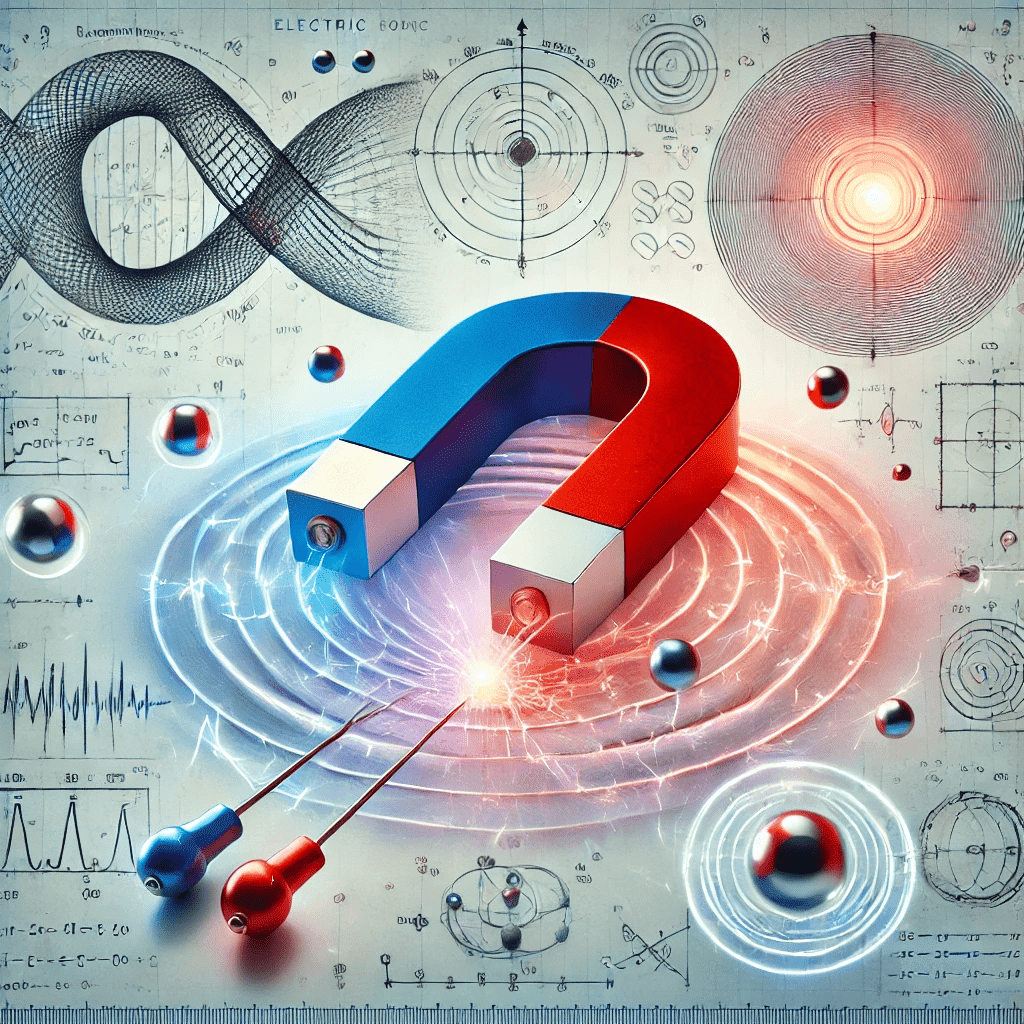
\includegraphics[width=2cm]{EMInteractions}};
\end{frame}

% ============================== Слайд ## ===================================
\begin{frame}{Зміст лекції}{}
	\tableofcontents
\end{frame}
% ===========================================================================



%% --------------------------------------------------------
\section{Означення}
%% --------------------------------------------------------



% ============================== Слайд ## ===================================
\begin{frame}{Означення}{}
	\begin{block}{}\justifying
		\href{https://www.youtube.com/watch?v=qS361iadCPA}{Дослід Ерстеда}, проведений 1820 року Ерстедом --- є першим експериментальним доказом впливу
		електричного струму на магніт (магнітну стрілку).
	\end{block}
	\begin{block}{}\justifying
		\alert{Магнітним полем} називається силове поле, що \alert{діє на рухомі заряди} і як наслідок --- на електричні струми  і на тіла, які мають
		магнітний  момент.
	\end{block}
	\begin{block}{}\justifying
		Магнітне поле створюється рухомими зарядами (електричним струмом). Незмінні в часі струми створюють постійні магнітні поля.
	\end{block}
	\begin{columns}
		\begin{column}{0.5\linewidth}\centering
			\begin{tikzpicture}[>=latex, scale=0.9, transform shape]
	\def\R{0.2}
	\draw[ball color=red!60] (0,0) circle (\R);
	\foreach \a in {20,40,...,340} {
			\draw[->, red] (0, 0) ++(\a:\R) -- (\a:1.5);
		}
	\draw[->, thick] (\R, 0) -- ++(2, 0) node[below] {$\vect{v}$};
	\draw[arrowpos={0.6}{2pt}{5pt}, blue, thick] (0,0) [partial ellipse=15:345:{0.3*0.5} and {1*0.5}];
	\draw[arrowpos={0.6}{2pt}{5pt}, blue, thick] (0,0) [partial ellipse=1:359:0.3 and 1];
	\draw[arrowpos={0.6}{2pt}{5pt}, blue, thick] (0,0) [partial ellipse=1:359:{0.3*1.5} and {1*1.5}];

	\foreach \c in {-1.5, +1.5}{
	\foreach \a in {0.2, 0.5, 1}{
	\draw[arrowpos={0.6}{2pt}{5pt}, blue, thick] (\c,0) [partial ellipse=1:359:{0.3*\a} and {1*\a}];
	}
	}
\end{tikzpicture}
		\end{column}
		\begin{column}{0.5\linewidth}
			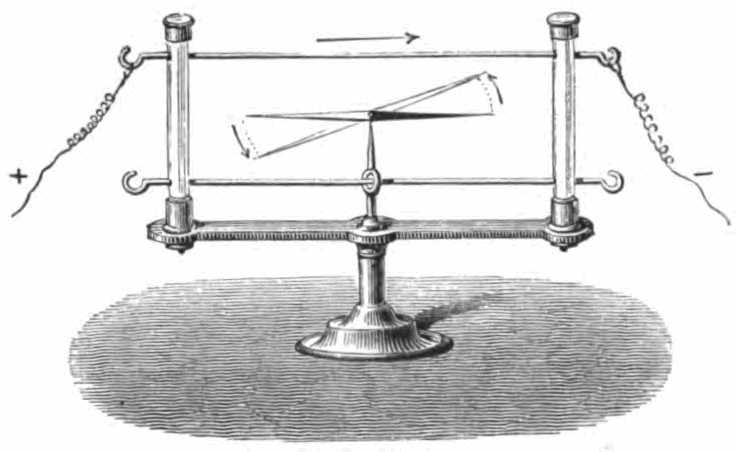
\includegraphics[width=0.9\linewidth]{OerstedExperiment}
		\end{column}
	\end{columns}
	\tikz[remember picture,overlay] \node[opacity=0.5,inner sep=0pt,
		anchor=north west] at (current page.north
	west){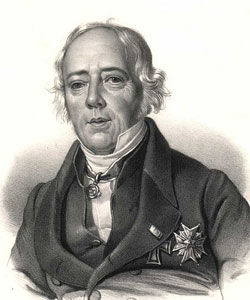
\includegraphics[width=2cm]{Ersted}};
\end{frame}
% ===========================================================================




%% --------------------------------------------------------
\section{Характеристика магнітного поля}
%% --------------------------------------------------------



% ============================== Слайд ## ===================================
\begin{frame}{Характеристика магнітного поля}{}
	\begin{block}{}\justifying
		Магнітних зарядів (магнітних монополів) у в природі немає (експериментальний факт). Характеристику магнітного поля, аналогічно до $\Efield =
			\frac{\vect{F}}{q}$
		ввести не можна. Однак в природі є магнітні диполі (магнітна стрілка, коловий виток зі струмом тощо), тому використовуючи аналогію з моментом
		сил, що діє на електричний диполь в електричному полі $ \vect{M} = \left[\vect{p}_e \times\Efield\right] $, можна ввести характеристику
		магнітного поля:
		\begin{equation*}
			\vect{M} = \left[\vect{p}_m \times\Bfield\right], \quad M_{\max} = p_m B
		\end{equation*}
		Характеристику магнітного поля, вектор $\Bfield$, по історичним причинам називають не \alert{напруженістю}, а \alert{індукцією} магнітного поля.
	\end{block}
	\begin{overprint}
		\onslide<1>
		\begin{block}{}\justifying
			Величина вектора індукції чисельно дорівнює максимальному обертальному моменту, що діє на одиничний магнітний момент вміщений у магнітне поле:
			\begin{equation*}
				B = \frac{\quad M_{\max}}{p_m}.
			\end{equation*}
		\end{block}
		\onslide<2>
		\begin{alertblock}{}\justifying
			В гауссовій системі одиниць величину магнітного поля називають Гаусом (Гс). С системі СІ Теслою (Тл):
			\begin{equation*}
				1\ \text{Тл} = 10^4\ \text{Гс}.
			\end{equation*}
		\end{alertblock}
	\end{overprint}
\end{frame}
% ===========================================================================



%% --------------------------------------------------------
\section{Дія магнітного поля на заряджені частинки та сруми}
%% --------------------------------------------------------



% ============================== Слайд ## ===================================
\begin{frame}{Сила Лоренца та сила Ампера}{}
	\begin{block}{}
		Магнітною складовою сили Лоренца називається сила, що діє на рухомий заряд $q$ з боку магнітного поля:
		\begin{equation*}
			\vect{F} = q\left[\frac{\vect{v}}{c}\times\Bfield\right].
		\end{equation*}
		Повна сила (власне і є сила Лоренца), що діє на заряд, включає також силу з боку електричного поля:
		\begin{equation*}
			\vect{F} = q\left( \Efield + \left[\frac{\vect{v}}{c}\times\Bfield\right] \right) .
		\end{equation*}
	\end{block}
	\begin{block}{}
		\alert{Силою Ампера} називають силу, що діє на струми з боку магнітного поля:
		\begin{equation*}
			d\vect{F} = \frac1c \left[ \vect{j}dV \times \Bfield\right],
		\end{equation*}
		де $\vect{j} dV$ --- називається \alert{елементом об'ємного струму}.
	\end{block}
\end{frame}
% ===========================================================================




% ============================== Слайд ## ===================================
\begin{frame}{Елемент струму}{}
	\begin{onlyenv}<1>
		\begin{columns}
			\begin{column}{0.3\linewidth}\centering
				\begin{tikzpicture}[>=latex,
		spy using outlines={circle, magnification=3, size=3.2cm, connect spies}
	]
	\draw[gray!60, line width=0.21cm] (0,0)  [partial ellipse=90:0:2];
	\fill[gray!50, draw = gray!70] (0, 2) circle (0.05 and 0.1);
	\fill[gray!50, rotate=-90, draw = gray!70] (0, 2) circle (0.05 and 0.1);

	\draw[red!40, line width=0.21cm] (0,0) [partial ellipse=55:45:2];
	\draw[{Latex[scale=0.5]}-{Latex[scale=0.5]}] (55:2.2)  arc(55:45:2.1) node[above=-1pt, sloped, pos=0.7, font=\tiny] {$d\ell$};
	\fill[red!40, draw = red!60, rotate=-45] (0, 2) coordinate (S1) circle (0.05 and 0.1);
	\fill[red!40, draw = red!60, rotate=-35] (0, 2)  circle (0.05 and 0.1);

	\node[font=\tiny, right, inner sep=0] (S) at (42:2.2) {$S$};

	\draw[{Latex[scale=0.3]}-, ultra thin] (S1) to[out=0] (S.west);

	\draw[-{Latex[scale=0.5]}, teal] (55:2)  node[below=1pt, text=teal, font=\tiny] {$\vect{j}$} -- ++({55-90}:0.2);
	\spy [gray] on (50:2.1)
	in node [] at (1.5,4.5);
\end{tikzpicture}
			\end{column}
			\begin{column}{0.7\linewidth}
				\begin{block}{}\justifying
					Якщо в задачі не цікавляться
					внутрішньою будовою провідника, та розподілом струму в його товщі, то можна ввести \alert{елемент лінійного струму}.
				\end{block}
				\begin{block}{}\justifying
					Нехай струм тече провідником із площею поперечного перерізу $S$. Уведемо вектор ділянки провідника завдовжки $d\vect{\ell}$
					за формулою $d\vect{\ell} = \vect{n}\ell$, де $\vect{n}$ --- одиничний вектор уздовж осі провідника. Тоді $\vect{j} = j\vect{n}$,
					а $I = j S$ і вираз для елемента об'ємного струму можна переписати у вигляді:
					\begin{equation*}
						\vect{j}dV = j\vect{n} S d\ell  = I d\vect{\ell}.
					\end{equation*}
				\end{block}
			\end{column}
		\end{columns}
		\begin{block}{}
			Для елемента лінійного струму сила Ампера:
			\begin{equation*}
				d\vect{F} = \frac1c \left[ I d\vect{\ell} \times \Bfield\right].
			\end{equation*}
		\end{block}
	\end{onlyenv}
	\begin{onlyenv}<2>
		\begin{tblr}{
			colspec={Q[c,h]X[j,m]}
			}
			\tikz[>=latex, baseline]{
    \draw[gray!60, line width=0.21cm] (0,0)  [partial ellipse=90:0:2];
    \fill[gray!50, draw = gray!70] (0, 2) circle (0.05 and 0.1);
    \fill[gray!50, rotate=-90, draw = gray!70] (0, 2) circle (0.05 and 0.1);

    \draw[red!40, line width=0.21cm] (0,0) [partial ellipse=55:45:2];
    \draw[{Latex[scale=0.5]}-{Latex[scale=0.5]}] (55:2.2)  arc(55:45:2.1) node[above=-1pt, sloped, pos=0.7, font=\tiny] {$d\ell$};
    \fill[red!40, draw = red!60, rotate=-45] (0, 2) coordinate (S1) circle (0.05 and 0.1);
    \fill[red!40, draw = red!60, rotate=-35] (0, 2)  circle (0.05 and 0.1);
    \node[font=\tiny, right, inner sep=0] (S) at (42:2.2) {$S$};
    \draw[{Latex[scale=0.3]}-, ultra thin] (S1) to[out=0] (S.west);
    \draw[-{Latex[scale=0.5]}, teal] (55:2)  node[below=1pt, text=teal, font=\tiny] {$\vect{j}$} -- ++({55-90}:0.2);
}
			 &
			Елемент об'ємного струму $\vect{j}dV$
			\\
			\tikz[>=latex, baseline]{
    \draw[gray!60, line width=0.05cm, arrowpos={0.2}{2pt}{6pt}] (0,0)  [partial ellipse=90:0:2] node[pos=0.2, anchor=north, text=black] {$I$};
    \draw[red!40, line width=0.05cm] (0,0) [partial ellipse=55:45:2];
    \draw[-{Latex[scale=0.5]}] (55:2)  arc(55:45:2) node[above, sloped, pos=0.7, font=\tiny] {$d\vect{\ell}$};
}
			 &
			Елемент лінійного струму $Id\vect{\ell}$
			\\
			\tikz[>=latex, baseline,
	pencildraw/.style={ %
			decorate,
			decoration={random steps,segment length=2pt,amplitude=1pt}
		},]{
	\draw[fill=gray!60] (0,0) -- ++(3, 0) decorate [pencildraw]
		{to ++(1, 1)}
	-- ++(-3, 0)
	decorate [pencildraw]  {to cycle};
	\foreach \s in {0.2,0.4,...,0.8}  {
			\draw[->, red] ({0.8+\s}, \s) -- ++(1.2, 0);
		}
	\draw (1.5, 0) -- node[right, fill=gray!60, circle, inner sep=0] {$l$} ++(1,1) node (S) [above=5pt] {$dS$};
	\draw[fill=red!50, opacity=0.5] (1.0,0) -- ++(1, 0) -- ++(1, 1) -- ++(-1, 0) -- cycle;
	\draw[->] (S.east) to[out=0, in=90] (2.7, 0.9);

}
			 &
			{
			Поверхнева густина струму $i = \frac{I}{l}$. \\
					Елемент струму $I\ell = il\ell = i S$, де $\ell$ та $l$ --- сторони виділеного елемента, площа якого $S = l\cdot \ell$.
					Елемент поверхневого струму $\vect{i}dS$
				}
		\end{tblr}
	\end{onlyenv}
\end{frame}
% ===========================================================================


% ============================== Слайд ## ===================================
\begin{frame}{Зв'язок сили Лоренца та сили Ампера}{}
	\begin{block}{}
		Сила Лоренца, що діє на заряд $dq$, дорівнює
		\begin{equation*}
			d\vect{F} = \left[\frac{dq \vect{v}}{c}\times\Bfield\right].
		\end{equation*}
		Оскільки $dq \vect{v} = \rho \vect{v} dV = \vect{j} dV$, то одразу отримуємо силу Ампера, що діє на об'ємний елемент струму:
		\begin{equation*}
			d\vect{F} = \frac1c \left[ \vect{j}dV \times \Bfield\right].
		\end{equation*}
		Для рухомого заряду $q$, що рухається з швидкістю $\vect{v}$ --- \alert{елементом струму струму є $q\vect{v}$}.
	\end{block}
	\begin{center}
		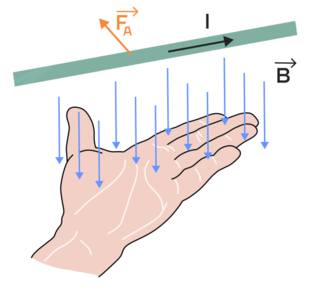
\includegraphics[width=2.2cm]{LeftHandRule}
	\end{center}
\end{frame}
% ===========================================================================



% ============================== Слайд ## ===================================
\begin{frame}{Робота магнітного поля}{}
	Робота сили Лоренца:
	\begin{columns}
		\begin{column}{0.65\linewidth}
			\begin{equation*}
				\delta A = \vect{F}\cdot d\vect{r} = \vect{F}\cdot\vect{v}dt = \left[\frac{q \vect{v}}{c}\times\Bfield\right] \cdot\vect{v}dt.
			\end{equation*}
			\begin{block}{}
				\begin{equation*}
					\vect{A}\cdot\vecdot{\vect{B}}{\vect{C}} = \vect{C}\cdot\vecdot{\vect{A}}{\vect{B}}.
				\end{equation*}
			\end{block}
			\begin{equation*}
				\vect{v}\cdot\left[\vect{v}\times\Bfield\right] = \Bfield\cdot\left[\vect{v}\times\vect{v}\right] = 0.
			\end{equation*}
			\begin{equation*}
				\delta A = 0.
			\end{equation*}
		\end{column}
		\begin{column}{0.35\linewidth}\centering
			\begin{tikzpicture}[>=latex, every node/.style={font=\scriptsize}, scale=1.4]
	\foreach \x in {0,...,2} {
			\draw[->, blue] (\x, 0) -- ++(0, 2) \ifnum\x=1 node[right] {$\Bfield$}\fi;
			\draw[->, blue] ({\x+0.5}, -0.5) -- ++(0, 2);
			\draw[arrowpos={0.2}{2pt}{5pt}, red] (1.25, 0.5) coordinate (O) [partial ellipse=360:0:1.2 and 0.2] node[pos=0.7, circle, inner
					sep=1pt, ball
					color=red,
					text=white] (q)
			{$+$} ;
		}
	\draw[->, green!50!black, thick] (q) -- ++(3:1) node[above] {$\vect{v}$};
	\draw[gray, ->] (q) -- (O) node[anchor=west] {$\vect{F}$};
\end{tikzpicture}
		\end{column}
	\end{columns}
	\begin{block}{}
		За теоремою про зміну кінетичної енергії $A = \Delta\left(\frac{mv^2}{2}\right) = 0$, кінетична енергія частинки не змінюється.
	\end{block}
	\begin{alertblock}{}\centering
		Магнітне поле не виконує роботи над частинкою!
	\end{alertblock}
\end{frame}
% ===========================================================================



%% --------------------------------------------------------
\section{Закон Біо-Савара-Лапласа}
%% --------------------------------------------------------



% ============================== Слайд ## ===================================
\begin{frame}{Закон Біо-Савара-Лапласа}{}
	\begin{block}{}\justifying
		Закон Біо-Савара встановлено експериментально (1820 р.) шляхом аналізу експериментальних даних і \alert{визначає магнітне поле, що створюється
			елементом струму}.
	\end{block}
	\begin{columns}
		\begin{column}{0.4\linewidth}\centering
			\begin{tikzpicture}[>=latex]
	\draw[gray!60, line width=0.21cm] (0,0)  [partial ellipse=90:0:2];
	\fill[gray!50, draw = gray!70] (0, 2) circle (0.05 and 0.1);
	\fill[gray!50, rotate=-90, draw = gray!70] (0, 2) circle (0.05 and 0.1);


	\foreach \n in {1,...,3} {
	\draw[rotate = -40, blue!40] (0, 2) [partial ellipse={10-2*\n}:{350+2*\n}:{0.2*\n} and \n];
	}

	\node[circle, fill, inner sep=0.5pt] (P) at (3.04,3) {};
	\node[below] at (P) {$P$};

	\draw[red!40, line width=0.21cm] (0,0)  [partial ellipse=55:45:2];
	\fill[red!40, draw = red!60, rotate=-45] (0, 2) circle (0.05 and 0.1);
	\fill[red!40, draw = red!60, rotate=-35] (0, 2) circle (0.05 and 0.1);
	\draw[-{Latex[scale=0.5]}] (55:2)  node[below=1pt] {$\vect{j}dV'$} -- ++({55-90}:0.2);
	\draw[-{Latex[scale=0.5]}] (50:2.1)  -- node[anchor=south, inner sep=1pt, sloped] {$\vect{\mathcal{r}}$} (P);
	\draw[->, blue, thick] (P) -- ++(63:0.75) node[anchor=225, text=black] {$d\Bfield$};

	%                \begin{scope}[opacity=0.5]
	%                    \coordinate (O) at (1.0, -0.5);
	%                    \draw[->, gray] (O) -- ++(1, 0);
	%    				\draw[->, gray] (O) -- ++(0, 1) ;
	%    				\draw[->, gray] (O) -- ++(225:0.75);
	%    				\draw[->, gray] (O) -- node[anchor=east, inner sep=3pt] {$\vect{r}'$} (50:1.9);
	%    				\draw[->, gray] (O) -- node[anchor=north, inner sep=3pt] {$\vect{r}$} (P);
	%                \end{scope}
\end{tikzpicture}
		\end{column}
		\begin{column}{0.6\linewidth}
			\begin{block}{}\justifying
				Якщо радіус-вектор точки спостереження відносно розглянутого елемента струму є $\vect{\mathcal{r}}$, то поле,
				створюване елементом струму $\vect{j} dV'$, дорівнює
				\begin{equation*}
					\tcbhighmath{d\Bfield = \frac1c \frac{\left[ \vect{j}dV'\times\vect{\mathcal{r}}\right] }{\mathcal{r}^3}.}
				\end{equation*}
			\end{block}
		\end{column}
	\end{columns}
	\begin{alertblock}{}
		Магнітне поле підкоряється принципу суперпозиції:
		\(
		\Bfield = \int d\Bfield.
		\)
	\end{alertblock}
\end{frame}
% ===========================================================================





% ============================== Слайд ## ===================================
\begin{frame}{Відносність величини магнітного поля}{}
	\begin{columns}
		\begin{column}{0.5\linewidth}
			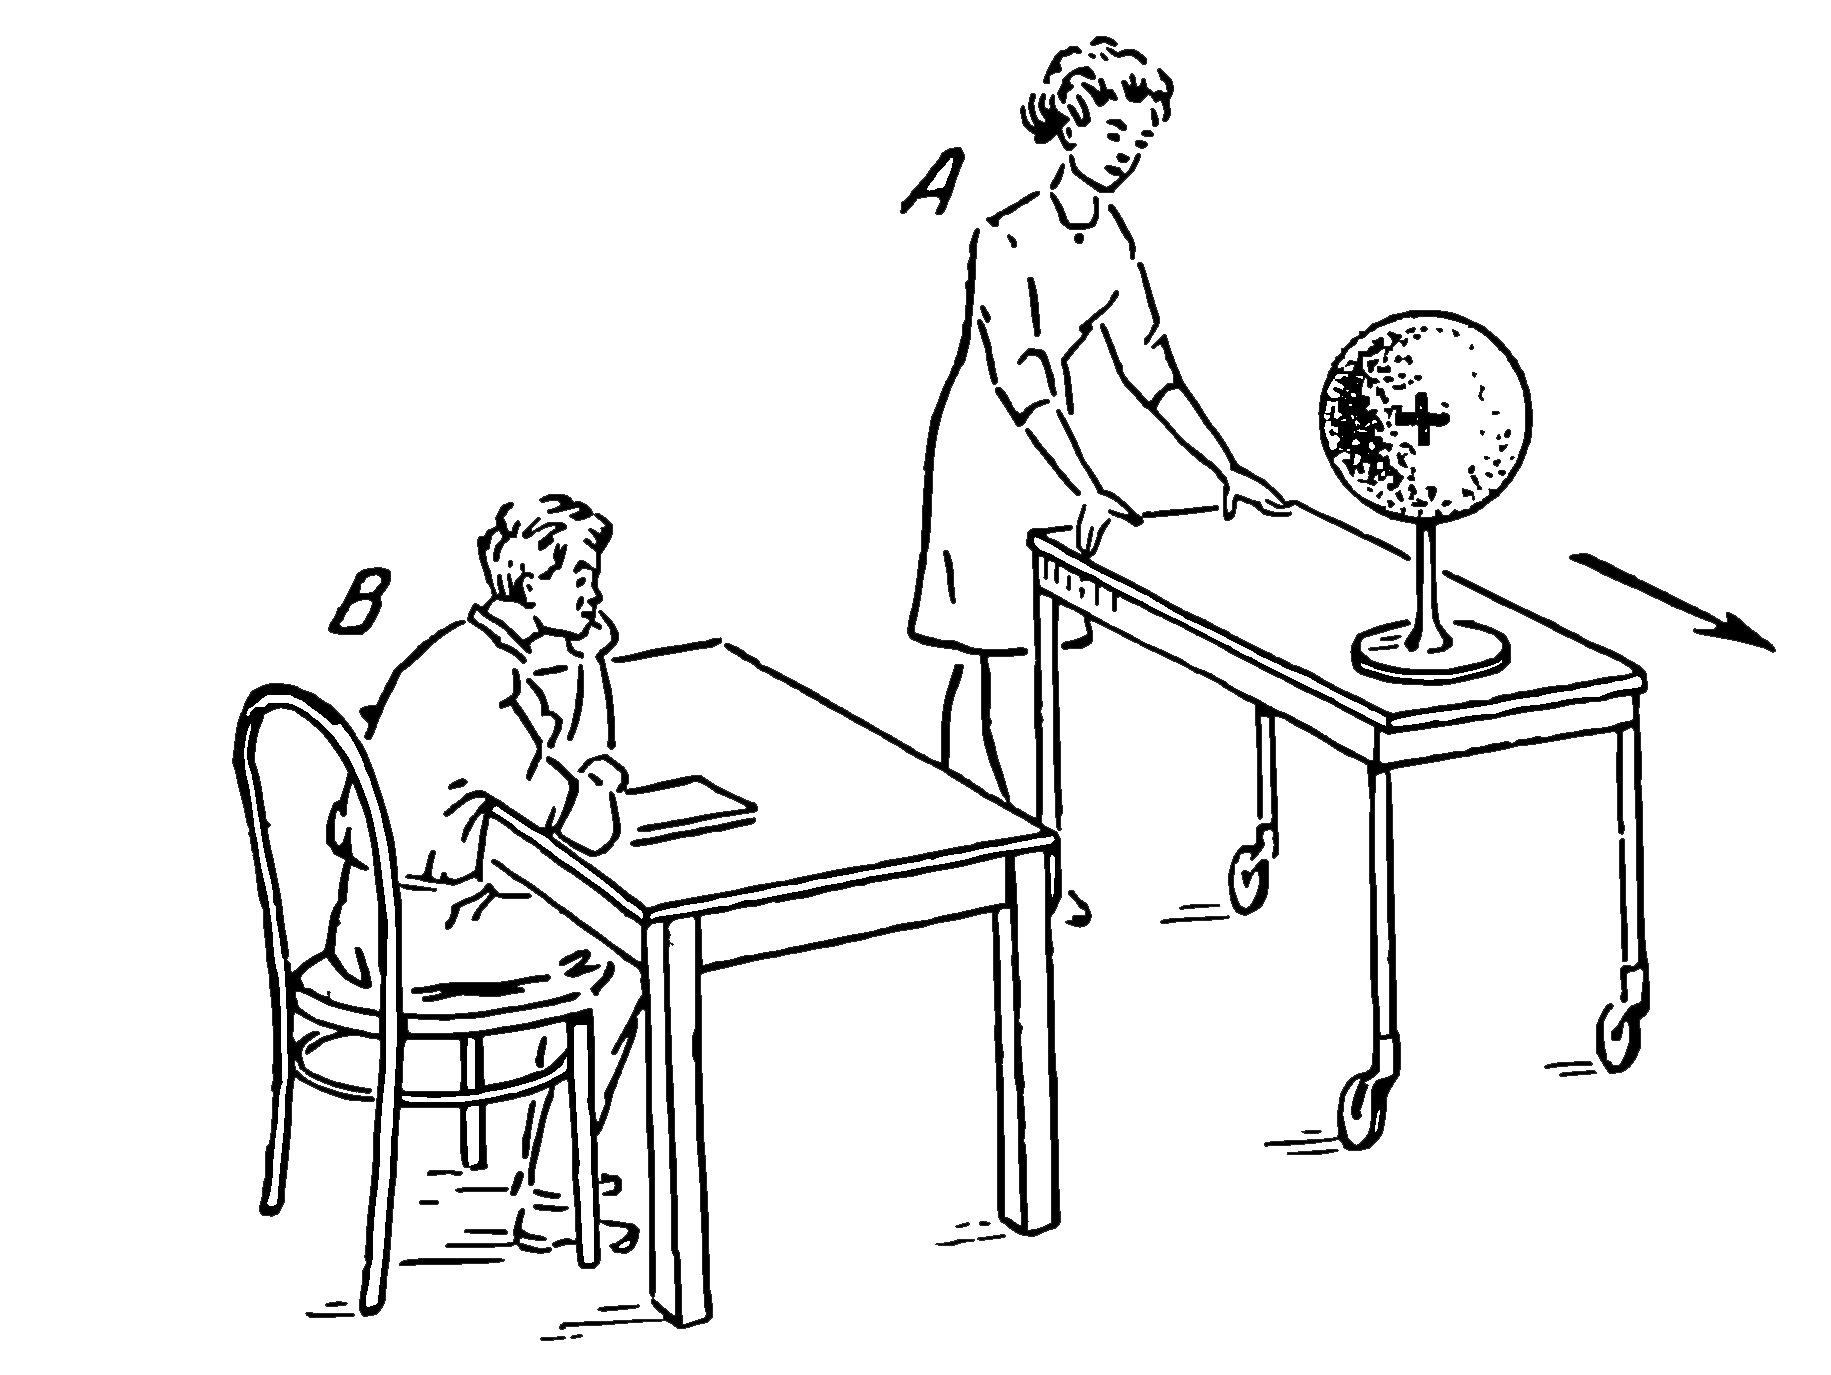
\includegraphics[width=0.85\linewidth]{MagFieldRelativity}
		\end{column}
		\begin{column}{0.5\linewidth}
			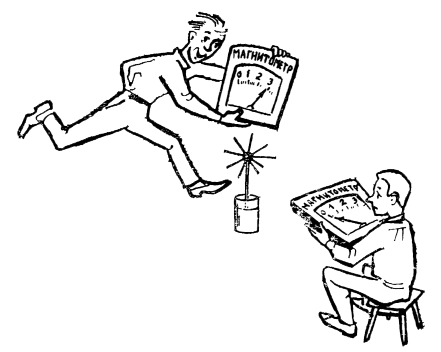
\includegraphics[width=0.85\linewidth]{MagFieldRelativity2}
		\end{column}
	\end{columns}
	\begin{block}{}
		Магнітного поля навколо заряду відносно спостерігача $A$ немає. Відносно спостерігача $B$ буде магнітне поле:
		\begin{equation*}
			\Bfield = \frac1c \frac{q\vect{v}\times\vect{\mathcal{r}}}{\mathcal{r}^3} =
			\frac{\vect{v}}{c}\times\frac{q\vect{\mathcal{r}}}{\mathcal{r}^3} = \frac{\vect{v}}{c}\times\Efield.
		\end{equation*}
	\end{block}
	\begin{alertblock}{}\centering
		Електричне і магнітне поле --- є прояв єдиного цілого, яке можна назвати \alert{електромагнітним полем}.
	\end{alertblock}
\end{frame}
% ===========================================================================


% ============================== Слайд ## ===================================
\begin{frame}{Приклади застосування закону Біо-Савара-Лапласа}{}
	%=========================================================
	\begin{exampleblock}{\scriptsize Задача 1}\label{prb:inf_wire}\justifying
		Визначити магнітне поле на відстані $r$ від нескінченно довгого провідника зі струмом $I$.
	\end{exampleblock}
	%=========================================================
	\begin{exampleblock}{\scriptsize Задача 2}\justifying
		Визначте магнітне поле в точці $P$ на відстані $r$ від короткого провідника зі струмом. Положення точки $P$ визначається кутами $\alpha_1$ та
		$\alpha_2$.
	\end{exampleblock}
	\begin{columns}
		\begin{column}{0.5\linewidth}\centering
			\begin{tikzpicture}[scale=0.75, transform shape]
				\draw[arrowpos={0.2}{0pt}{5pt}, line width=1pt, gray] (0, 0)  to  +(0, 4) coordinate (B);
				\draw[densely dotted, line width=1pt, gray] (B) -- +(0,0.5) (0,0) -- +(0,-0.5);
				\draw[blue!40, arrowpos={0.5}{0pt}{5pt}] (0, 1.75) [partial ellipse=110:{360+70}:{1.5} and 0.2];
				\draw[-latex] (0, 1.75) -- node [below] {$\vect{r}$} ++(1.5, 0);
			\end{tikzpicture}
		\end{column}
		\begin{column}{0.5\linewidth}\centering
			\begin{tikzpicture}[scale=0.75, transform shape]
				\draw[arrowpos={0.2}{0pt}{5pt}, line width=1pt, gray] (0,0) --  +(0,4) coordinate (B) node[contact] {};
				\draw[densely dotted, line width=1pt, gray] (B) -- +(0,1) (0,0) -- +(0,-1);
				\draw[blue!40, arrowpos={0.5}{0pt}{5pt}] (0, 1.75) [partial ellipse=110:{360+70}:{1.5} and 0.2];
				\draw[-latex] (0, 1.75) -- node [below]  {$\vect{r}$} ++(1.5, 0) coordinate (P);
				\draw (0, 0) -- (P);
				\draw (0, 0) ++(0, 0.2) arc (90:{90-atan(1.5/1.75)}:0.2) node[pos=1, anchor=west] {$\alpha_1$};

				\draw (B) -- (P);
				\draw (B) ++(0, 0.5) arc (90:{-90+atan(1.5/2.25)}:0.5) node[pos=0.5, anchor=west] {$\alpha_2$};
			\end{tikzpicture}
		\end{column}
	\end{columns}
\end{frame}
% ===========================================================================


% ============================== Слайд ## ===================================
\begin{frame}{Взаємодія струмі}{Досліди Ампера}
	\begin{block}{}\justifying
		У 1820 р. А. Ампером було встановлено закон, що визначає силу, яка діє на елемент струму в магнітному полі. Оскільки створити відокремлений елемент
		не можна, то Ампер вивчав вплив паралельних дротів один на одного та поведінку дротяних замкнутих контурів різної форми в магнітному полі.
	\end{block}
	\tikz[remember picture,overlay] \node[opacity=0.5,inner sep=0pt,
		anchor=north west] at (current page.north
	west){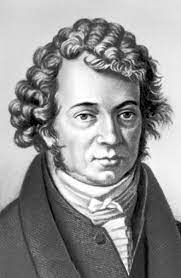
\includegraphics[width=2cm]{Ampere}};
	\begin{columns}
		\begin{column}{0.5\linewidth}\centering
			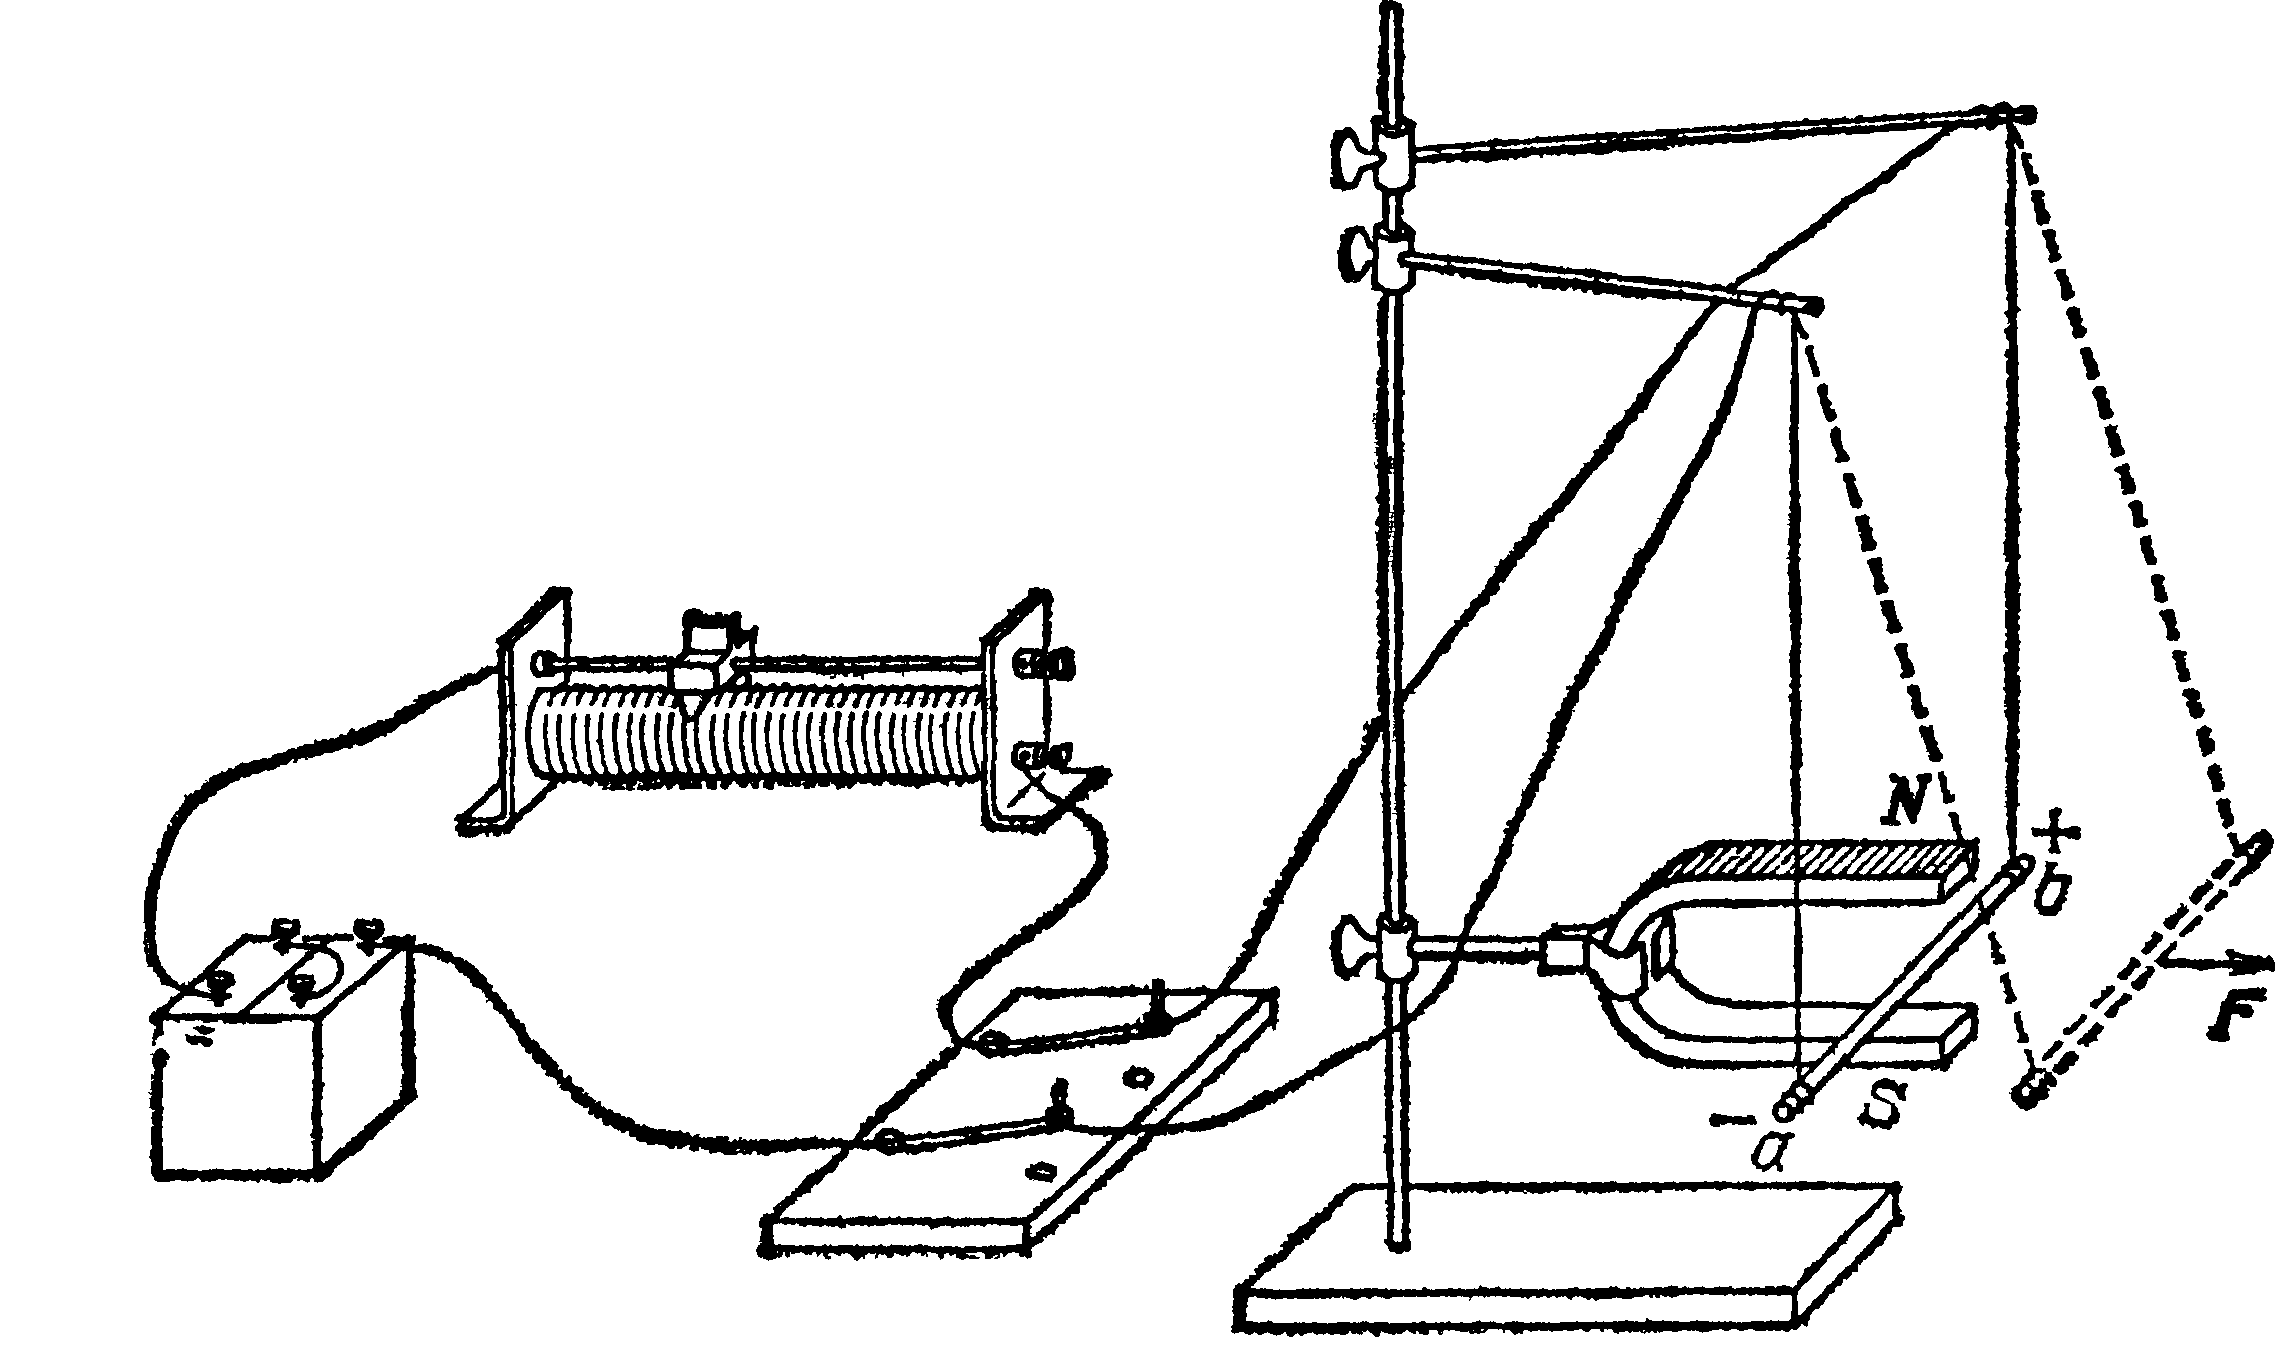
\includegraphics[width=\linewidth]{AmpereForce1}
		\end{column}
		\begin{column}{0.5\linewidth}\centering
			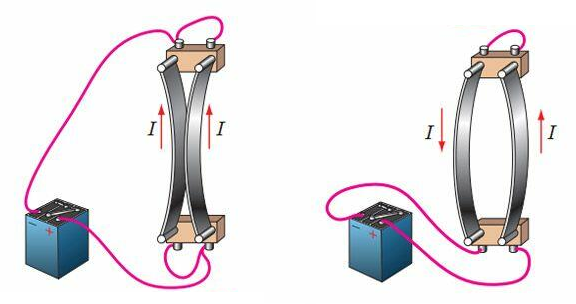
\includegraphics[width=\linewidth]{AmpereForce2}
		\end{column}
	\end{columns}
\end{frame}
% ===========================================================================

%% --------------------------------------------------------
\section{Вектор-потенціал магнітного поля}
%% --------------------------------------------------------


% ============================== Слайд ## ===================================
\begin{frame}[t]{Вектор-потенціал магнітного поля}{}
	\framesubtitle<1>{Введення поняття}
	\framesubtitle<2>{Калібруванні вектор-потенціалу}
	\begin{columns}
		\begin{column}{0.3\linewidth}\centering
			\begin{tikzpicture}[>=latex]
	\draw[gray!60, line width=0.21cm] (0,0)  [partial ellipse=90:0:2];
	\fill[gray!50, draw = gray!70] (0, 2) circle (0.05 and 0.1);
	\fill[gray!50, rotate=-90, draw = gray!70] (0, 2) circle (0.05 and 0.1);

	\node[circle, fill, inner sep=0.5pt] (P) at (2.5,3) {};
	\node[above] at (P) {$P$};

	\draw[red!40, line width=0.21cm] (0,0)  [partial ellipse=80:70:2];
	\fill[red!40, draw = red!60, rotate=-10] (0, 2) circle (0.05 and 0.1);
	\fill[red!40, draw = red!60, rotate=-20] (0, 2) circle (0.05 and 0.1);
	\draw[-{Latex[scale=0.5]}] (80:2)  node[above=1pt] {$\vect{j}$} -- ++({80-90}:0.2);
	\draw[->] (75:2.1)  -- (P) node[anchor=south east, inner sep=1pt, sloped, pos=0.8] {$\vect{r} - \vect{r}'$} ;
	%                \draw[->, blue, thick] (P) -- ++(63:0.75) node[anchor=225, text=black] {$d\Bfield$};

	\draw[->] (0, 0) -- ++(1, 0) node[below] {$y$};
	\draw[->] (0, 0) -- ++(0, 1) node[left] {$z$};
	\draw[->] (0, 0) -- ++(225:0.75) node[left] {$x$};
	\draw[->] (0,0) -- node[anchor=west, inner sep=3pt] {$\vect{r}'$} (75:1.8);
	\draw[->] (0,0) -- node[anchor=north, inner sep=3pt] {$\vect{r}$} (P);
\end{tikzpicture}
		\end{column}
		\begin{column}{0.7\linewidth}
			\begin{overprint}
				\onslide<1>
				\begin{block}{}
					Закон Біо-Савара-Лапласа
					\begin{equation*}
						\Bfield(\vect{r}) = \iiint\limits_{V'} \frac1c \frac{ \vect{j}(\vect{r}')dV'\times(\vect{r} - \vect{r}') }{|\vect{r} -
							\vect{r}'|^3}
					\end{equation*}
					{\small
					Використаємо тотожність:
					\(
					\frac{ (\vect{r} - \vect{r}') }{|\vect{r} - \vect{r}'|^3} = - \vect{\nabla}_{\vect{r}} \frac{ 1 }{|\vect{r} - \vect{r}'|},
					\)
					у якому операція $\vect{\nabla}$ діє на координати $\vect{r}$, а також рівність
					$\Rot(\phi\vect{C}) = \phi\Rot\vect{C} + \vecdot{\grad\phi}{\vect{C}} $.}
				\end{block}
				\onslide<2>
				\begin{block}{}
					\begin{equation*}
						\tcbhighmath{\Bfield = \Rot\vect{A},}
					\end{equation*}
					Введений тут вектор $\vect{A}$ називається \alert{вектор-потенціалом}:
					\begin{equation*}
						\vect{A}(\vect{r}) = \frac1c \int\limits_{V'} \frac{\vect{j}(\vect{r}')}{|\vect{r} - \vect{r}'|} dV',
						\
						\vect{A}(\vect{r}) = \frac1c \sum\limits_i \frac{q_i\vect{v}_i}{|\vect{r} - \vect{r}_i|}
					\end{equation*}
				\end{block}
			\end{overprint}
		\end{column}
	\end{columns}
	\begin{overprint}
		\onslide<1>
		\begin{block}{}
			\begin{equation*}
				\Bfield(\vect{r}) =\int\limits_{V'} \frac1c \vect{\nabla} \frac{ 1 }{|\vect{r} - \vect{r}'|}\times\vect{j} (\vect{r}') dV'  =
				%
				\Rot \frac1c \int\limits_{V'} \frac{\vect{j}dV'}{|\vect{r} - \vect{r}'|}  = \Rot\vect{A}(\vect{r}),
			\end{equation*}
			\begin{equation*}
				\Bfield(\vect{r}) = \Rot\vect{A}(\vect{r}).
			\end{equation*}
		\end{block}
		\onslide<2>
		\begin{block}{}\justifying\small
			\alert{Вектор-потенціал вводиться при цьому неоднозначно}.
			Векторні потенціали $\vect{A}$ і $\vect{A}' = \vect{A} + \grad f(\vect{r})$
			призводять до одного й того ж магнітного поля $\Bfield$. Цією обставиною можна
			скористатися для того, щоб накласти на $\vect{A}$ яке-небудь обмеження. Зручно накласти на $\vect{A}$ умову
			\begin{equation*}
				\tcbhighmath{\Div\vect{A} = 0,} \quad \text{\color{red}кулонівське калібрування}.
			\end{equation*}
		\end{block}
	\end{overprint}
\end{frame}
% ===========================================================================


%% --------------------------------------------------------
\section{Теореми магнітостатики}
%% --------------------------------------------------------




% ============================== Слайд ## ===================================
\begin{frame}{Теорема Гаусса для магнітного поля}{}
	Маючи на увазі тотожність $\Div\Rot\vect{A} = 0$, з формули $\Bfield = \Rot\vect{A}$ отримуємо теорему Гауса в диференціальній формі:
	\begin{equation*}
		\tcbhighmath{\Div\Bfield = 0}
	\end{equation*}
	Застосовуючи теорему Остроградського-Гауса отримуємо теорему Гауса в інтегральній формі:
	\begin{equation*}
		\tcbhighmath{\oiint\limits_S \Bfield\cdot d\vect{S} = 0.}
	\end{equation*}
	\begin{alertblock}{}\justifying
		Теорема Гауса стверджує, що немає вільних (незв'язаних) магнітних зарядів, на яких могли б починатися або закінчуватися силові лінії індукції
		магнітного поля.
	\end{alertblock}

\end{frame}
% ===========================================================================


% ============================== Слайд ## ===================================
\begin{frame}{Теорема про циркуляцію магнітного поля у вакуумі}{Диференціальна форма}
	\begin{block}{}
		Знайдемо ротор вектора $\Bfield$:
		\begin{equation*}
			\Rot\Bfield = \Rot\Rot\vect{A} = \rot\vecdot{\grad}{\vect{A}}  = \grad\scdot{\grad}{\vect{A}} - \nabla^2\vect{A}
			\stackrel{\color{red}\divg\vect{A}
				= 0}{=}  - \nabla^2\vect{A}.
		\end{equation*}
	\end{block}
	\begin{exampleblock}{\small Аналогія з рівнянням Пуассона з електростатики}\small
		Рівняння Пуассона та його розв'язок:
		\begin{equation*}
			\nabla^2\phi= -4\pi\rho,\ \phi = \iiint\limits_{V'} \frac{\rho dV'}{|\vect{r} - \vect{r}'|}, \qquad
			\nabla^2 \vect{A} = -\frac{4\pi}{c} \vect{j},\
			\vect{A} = \frac1c\iiint\limits_{V'} \frac{\vect{j} dV'}{|\vect{r} - \vect{r}'|}
		\end{equation*}
		\begin{center}
			\alert{Однакові рівняння мають однакові розв'язки!}
		\end{center}
	\end{exampleblock}
	\begin{block}{}\centering
		Теорема про циркуляцію для вектора $\Bfield$:
		\begin{equation*}
			\tcbhighmath{\Rot\Bfield = \frac{4\pi}c\vect{j}.}
		\end{equation*}
	\end{block}
\end{frame}
% ===========================================================================



% ============================== Слайд ## ===================================
\begin{frame}{Теорема про циркуляцію магнітного поля у вакуумі}{Інтегральна форма}
	\begin{block}{}
		Циркуляція вектора $\Bfield$ по довільному контуру $L$ пропорційна струмам, що охоплюються контуром $L$.
	\end{block}
	\begin{columns}\centering
		\begin{column}{0.5\linewidth}
			\begin{equation*}
				\tcbhighmath{\oint\limits_{L}\Bfield\cdot d\vect{r} = \frac{4\pi}c \iint\limits_{S} \vect{j}\cdot d\vect{S}.}
			\end{equation*}
		\end{column}
		\begin{column}{0.5\linewidth}\centering
			\begin{tikzpicture}[>=latex, scale=0.7, transform shape]
				\draw [in=-105, out=75, looseness=1.25, line width=4pt, gray!50] (-1, -1) coordinate (A) to (2, 2) coordinate (B);
				\draw[fill=gray!50, ultra thin, rotate around={-10:(B)}] (B) circle(2pt and 0.75pt);
				\draw[fill=gray!50, ultra thin, rotate around={-10:(A)}] (A) circle(2pt and 0.75pt);
				\draw[thick, green!50!black] (0, 0) circle(1 and 0.3);
				\begin{scope}
					\clip (0,0) rectangle (1,1);
					\draw [in=-105, out=75, looseness=1.25, line width=4pt, gray!50] (-1, -1) coordinate (A) to (2, 2) coordinate (B);
				\end{scope}
				\draw[red!20, pattern=crosshatch, pattern color=red!20] (-1,0) to[out=85, in=45, looseness=3] node[pos=0.2, above, text=red]
				{$S$} (1, 0) arc(0:-180:1 and 0.3) ;
				\draw[thick, arrowpos={0.5}{3pt}{4pt}, green!50!black] (-1, 0) arc(180:360:1 and 0.3) node[pos=0.5, below] {$L$};
			\end{tikzpicture}
		\end{column}
	\end{columns}
	\begin{block}{}\justifying
		У випадку дискретних струмів, циркуляція вектора $\Bfield$ по довільному контуру $L$ пропорційна алгебраїчній сумі струмів, що охоплюються
		контуром~$L$.
	\end{block}
	\begin{columns}
		\begin{column}{0.5\linewidth}
			\begin{equation*}
				\tcbhighmath{\oint\limits_{L}\Bfield\cdot d\vect{r} = \frac{4\pi}c \sum\limits_i I_i.}
			\end{equation*}
		\end{column}
		\begin{column}{0.5\linewidth}\centering
		\begin{tikzpicture}[>=latex]
			\draw [arrowpos={0.9}{2pt}{4pt}, in=-45, out=45, looseness=1.25, line width=1pt, gray!50] (-1, -1) to (-1, 1) node[above, text=black] {$I_1 >
					0$};
			\draw [arrowpos={0.1}{2pt}{4pt}, out=225, looseness=0.80, line width=1pt, gray!50] (0.2, 1) node[above, text=black ] {$I_2 < 0$} to (0.2,
			-1) ;
			\draw [arrowpos={0.1}{2pt}{4pt}, line width=1pt, gray!50]  (0.9, 0.1)  circle(0.2 and 0.7) node[above right=0.4cm, text=black] {$I_3 <
						0$};
			\draw[thick, green!50!black, fill=red!20] (0, 0) circle(1 and 0.3);
			\draw[thick, arrowpos={0.4}{3pt}{4pt}, green!50!black] (-1, 0) arc(180:360:1 and 0.3) node[pos=0.4, below] {$L$};
            \draw[->, red, thick] (0,0) -- ++(0, 0.5);
			\node[text=red] at (0.3, 0) {$S$};
			\begin{scope}
				\clip (-1, 0) rectangle ++(2, 0.5);
				\draw [in=-45, out=45, looseness=1.25, line width=1pt, gray!50] (-1, -1) to (-1, 1);
				\draw [out=225, looseness=0.80, line width=1pt, gray!50] (0.2, 1)  to (0.2, -1);
				\draw [line width=1pt, gray!50]  (0.9, 0.1)  circle(0.2 and 0.7);
			\end{scope}
            \node[rotate=90] at (-1.5, 0) {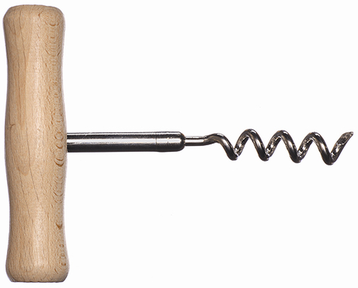
\includegraphics[width=1cm]{corksckrew.png}};
		\end{tikzpicture}
		\end{column}
	\end{columns}
\end{frame}
% ===========================================================================

% ============================== Слайд ## ===================================
\begin{frame}{Приклади на теорему про циркуляцію \No 1}{}
	\begin{equation*}
		\oint\limits_{L}\Bfield\cdot d\vect{r} = \frac{4\pi}c \sum_i I_i
	\end{equation*}
	\begin{overprint}
		\onslide<1>
		\begin{center}\small
			\begin{tblr}%
				{colspec={c|c}}
				\tikz[>=latex]{
				\node [] (0) at (0, -1) {};
				\node [] (1) at (0, +1) {};
				\draw[line width=2pt, gray, arrowpos={0.7}{4pt}{7pt}] [in=-45, out=120, looseness=1.25] (0.center) to (1.center);
				\foreach \n in {1,...,4} {
				\draw[blue!40, arrowpos={0.2}{0pt}{2pt}] (0, 0) [partial ellipse=90:430:{0.3*\n} and {0.05*\n}] ;
				}
				\draw[thin, green!50!black, arrowpos={0.2}{0pt}{2pt}] (0,0) [partial ellipse=90:440:{0.3*5} and {0.05*5}]
				node[pos=0.2, above] {$L$};
				}
				 &
				\tikz[>=latex]{
				\node [] (0) at (0, -1) {};
				\node [] (1) at (0, +1) {};
				\draw[line width=2pt, gray, arrowpos={0.7}{4pt}{7pt}] [in=-45, out=120, looseness=1.25] (0.center) to (1.center);
				\foreach \n in {1,...,4} {
				\draw[blue!40, arrowpos={0.2}{0pt}{2pt}] (0, 0) [partial ellipse=90:430:{0.3*\n} and {0.05*\n}] ;
				}
				\draw[thin, green!50!black, arrowpos={0.2}{0pt}{2pt}] (-1,0) [partial ellipse=0:360:{0.3*2} and {0.05*2}]
				node[pos=0.2, above] {$L$};
				}
				\\
				$\oint\limits_L \Bfield\cdot d\vect{r} = \frac{4\pi}c I$
				 &
				$\oint\limits_L \Bfield\cdot d\vect{r} = 0$
				\\\hline
				\tikz[>=latex]{
				\node [] (0) at (0, -1) {};
				\node [] (1) at (0, +1) {};
				\draw[line width=2pt, gray, arrowpos={0.7}{4pt}{7pt}] [in=-45, out=120, looseness=1.25] (0.center) to (1.center);
				\draw[line width=2pt, gray, arrowpos={0.7}{4pt}{7pt}] [out=-45, in=120, looseness=1.25] ([xshift=0.5cm]1.center) to
				([xshift=0.5cm]0.center);
				\draw[thin, green!50!black, arrowpos={0.4}{0pt}{2pt}] (-0.5,0) [partial ellipse=0:360:{0.3*3} and {0.05*3}]
				node[pos=0.4, above] {$L$};
				}
				 &
				\tikz[>=latex]{
				\node [] (0) at (0, -1) {};
				\node [] (1) at (0, +1) {};
				\draw[line width=2pt, gray, arrowpos={0.7}{4pt}{7pt}] [in=-45, out=120, looseness=1.25] (0.center) to (1.center);
				\draw[line width=2pt, gray, arrowpos={0.7}{4pt}{7pt}] [out=-45, in=120, looseness=1.25] ([xshift=0.5cm]1.center) to
				([xshift=0.5cm]0.center);
				\draw[thin, green!50!black, arrowpos={0.4}{0pt}{2pt}] (-0.1,0) [partial ellipse=0:360:{0.3*3} and {0.05*3}]
				node[pos=0.4, above] {$L$};
				}  \\
				$\oint\limits_L \Bfield\cdot d\vect{r} = \frac{4\pi}c I$
				 &
				$\oint\limits_L \Bfield\cdot d\vect{r} = \frac{4\pi}c (I + (-I)) = 0$
				\\
			\end{tblr}
		\end{center}
		\onslide<2>
		\begin{tblr}{colspec={Q[c,m, 0.3\linewidth]|X[c,m]}}
			Поле нескінченного провідника
			 &
			\tikz[>=latex, baseline]{
			\node [] (0) at (0, -1) {};
			\node [] (1) at (0, +1) {};
			\draw[line width=2pt, gray, arrowpos={0.7}{4pt}{7pt}] (0.center) to (1.center);
			\foreach \n in {1,...,4} {
			\draw[blue!40, arrowpos={0.2}{0pt}{2pt}] (0, 0) [partial ellipse=100:435:{0.3*\n} and {0.05*\n}] ;
			}
			\draw[thin, green!50!black, arrowpos={0.2}{0pt}{2pt}] (0,0) [partial ellipse=100:435:{0.3*4} and {0.05*4}]
			node[pos=0.2, above] {$L$};
			}
			$
				B = \dfrac{2I}{c r}
			$
			\\\hline
			Поле нескінченного соленоїда
			 &
			\tikz[>=latex, baseline]{
			\foreach \y in {-1,-0.85,...,1} {
			\draw[thin, gray, arrowpos={0.4}{0pt}{4pt}] (0,\y) [partial ellipse=100:450:{0.3*4} and {0.05*4}];
			}
			\draw [thin, green!50!black, arrowpos={0.6}{0pt}{4pt}] (0,-0.5) rectangle (2,0.5) node[pos=0.6, right] {$L$};
			}
			$
				B = \frac{4\pi}c\frac{N}{l} I
			$
		\end{tblr}
	\end{overprint}
\end{frame}
% ===========================================================================



% ============================== Слайд ## ===================================
\begin{frame}{Приклади на теорему про циркуляцію \No 2}{}
	\begin{equation*}
		\oint\limits_{L}\Bfield\cdot d\vect{r} = \frac{4\pi}c \iint\limits_{S} \vect{j}\cdot d\vect{S}
	\end{equation*}
	\begin{center}\small
		\begin{tblr}%
			{colspec={Q[c,m, 0.3\linewidth]|X[l,m]}}
			Поле всередині нескінченного циліндричного провідника
			 &
			\tikz[>=latex, baseline]{
			\draw[gray!50, line width=1cm] (0, -1) -- (0,1);
			\draw[] (-0.5, -1) -- (-0.5,1) (+0.5, -1) -- (+0.5,1) ;
			\draw[fill=gray!50] (0,1) circle (0.5 and 0.1);
			\draw[fill=gray!50] (0,-1) ++(-0.5,0) arc (180:360:0.5 and 0.1);
			\draw[dotted] (0,-1) ++(+0.5,0) arc (0:180:0.5 and 0.1);
			\draw[thin, green!50!black, arrowpos={0.1}{0pt}{2pt}, fill=green] (0,0) [partial ellipse=0:360:{0.3*1} and {0.05*1}]
			node[pos=0.1, above] {$L$};
			\draw[->] (0,-0.1) -- ++(0, 0.5) node[left] {$\vect{j}$};
			\path  (0,0) [partial ellipse=0:360:{0.3*3} and {0.05*3}];
			}
			$
				B = \dfrac{2\pi}c jr
			$
			\\\hline
			Поле зовні нескінченного циліндричного провідника
			 &
			\tikz[>=latex, baseline]{
			\draw[gray!50, line width=1cm] (0, -1) -- (0,1);
			\draw[] (-0.5, -1) -- (-0.5,1) (+0.5, -1) -- (+0.5,1) ;
			\draw[fill=gray!50] (0,1) circle (0.5 and 0.1);
			\draw[fill=gray!50] (0,-1) ++(-0.5,0) arc (180:360:0.5 and 0.1);
			\draw[dotted] (0,-1) ++(+0.5,0) arc (0:180:0.5 and 0.1);
			\draw[thin, green!50!black, arrowpos={0.1}{0pt}{2pt}] (0,0) [partial ellipse=0:360:{0.3*3} and {0.05*3}]
			node[pos=0.1, above] {$L$};

			\fill[green] (0,0) [partial ellipse=0:360:{0.5} and {0.05}];

			\draw[->] (0,-0.1) -- ++(0, 0.5) node[left] {$\vect{j}$};
			}
			$
				B = \dfrac{2}{cr} j\pi R^2 = \dfrac{2I}{cr}
			$
		\end{tblr}
	\end{center}

\end{frame}
% ===========================================================================


% ============================== Слайд ## ===================================
\begin{frame}{Порівняння законів \\електро- та магнітостатики у вакуумі}{}

	\begin{center}
		Диференціальні теореми\\[1ex]

		\begin{tblr}%
			{
			colspec={|Q[l,m, 1.6cm, bg=yellow! 10]|[1pt, white]Q[c,m, bg=red! 10]|Q[c,m, 1.5cm, font=\tiny]|[1pt, white]Q[c,m,
			bg=blue! 10]|Q[c,m,1.5cm,
			font=\tiny]|},
			row{1}={c, fg=white, bg=cyan, font=\bfseries},
			%hlines,
			}
			\hline
			Теорема                    & Електростатика                  & Зміст                                  & Магнітостатика                       &
			Зміст                                                                                                                                                                         \\
			\hline
			Зв'язок потенціалу та поля & $\Efield = -\grad\phi$          & Скалярний потенціал, поле потенціальне & $\Bfield  = \rot\vect{A}$
			                           & Вектор-потенціал. Поле вихрове.                                                                                                                  \\\hline
			Теорема Гаусса             & $\Div\Efield = 4\pi\rho$        & Джерелами поля є електричні заряди     & $\Div\Bfield = 0$                    & Джерел у магнітного поля немає \\
			\hline
			Теорема про циркуляцію     & $\Rot\Efield = 0$               & Електростатичне поле є потенціальним   & $\Rot\Bfield = \frac{4\pi}c\vect{j}$ & Магнітне поле є
			вихровим. Вихором є струм.                                                                                                                                                    \\
			\hline
		\end{tblr}
	\end{center}

	\begin{center}
		Інтегральні теореми\\[1ex]

		\begin{tblr}%
			{
			colspec={|Q[l,m, 1.6cm, bg=yellow! 10]|[1pt, white]Q[c,m, bg=red! 10, 4.08cm]|[1pt, white]Q[c,m, bg=blue! 10, 4.08cm]|},
			row{1}={c, fg=white, bg=cyan, font=\bfseries},
			%hlines,
			}
			\hline
			Теорема                & Електростатика                                                            &
			Магнітостатика                                                                                                                                              \\
			\hline
			Теорема Гаусса         & $\oiint\limits_S \Efield\cdot d\vect{S} = 4\pi \iiint\limits_{V} \rho dV$ & $\oiint\limits_S\Bfield\cdot d\vect{S} = 0 $           \\
			\hline
			Теорема про циркуляцію & $ \oint\limits_L\Efield\cdot d\vect{r} = 0 $                              & $\oint\limits_{L}\Bfield\cdot d\vect{r} = \frac{4\pi}c
				\iint\limits_{S}
			\vect{j}\cdot d\vect{S} $                                                                                                                                   \\
			\hline
		\end{tblr}
	\end{center}

\end{frame}
% ===========================================================================



%% --------------------------------------------------------
\section{Магнітний момент}
%% --------------------------------------------------------



% ============================== Слайд ## ===================================
\begin{frame}{Магнітний момент}{}
	\begin{alertblock}{}\centering
		Моменту імпульсу $\vect{L} = \vect{r}\times(m\vect{v}) $ для руху мас є аналогом магнітного моменту для руху зарядів!
	\end{alertblock}
	\begin{tblr}{
		colspec={X[c,m, mode=dmath]X[c,m, mode=dmath]},
		row{1}={mode=text, font=\bfseries\small},
		}
		Момент імпульсу                                                           & Магнітний момент                                      \\
		\tcbhighmath{\vect{L} = \iiint\limits_{V} \vect{r}\times\rho\vect{v}\ dV} & \tcbhighmath{\vect{p}_m = \frac1{2c}\iiint\limits_{V}
			\vect{r}\times\rho\vect{v}\ dV}
	\end{tblr}
	\begin{block}{}\justifying\small
		Оскільки густина струму $\vect{j} = \rho\vect{v}$, а $\vect{j} dV$ --- є елементом струму, то можна для різних випадків записати різні
		варіації
		формули магнітного моменту:
	\end{block}
	\begin{center}\scriptsize
		\begin{tblr}{
			colspec={Q[c,m, 0.4\linewidth]X[c,m, mode=dmath]},
			row{1}={mode=text, font=\bfseries\small, fg=white, bg=cyan, font=\bfseries},
			hlines,
			vlines,
			}
			Випадок                          & Магнітний момент                                                       \\
			Об'ємні струми                   & \vect{p}_m = \frac1{2c}\iiint\limits_{V} \vect{r}\times\vect{j} dV     \\
			Лінійні замкнені постійні струми & \vect{p}_m = \frac{I}{2c}\oint\limits_{L}  \vect{r}\times d\vect{\ell} \\
		\end{tblr}
	\end{center}
\end{frame}
% ===========================================================================



%% ============================== Слайд ## ===================================
\begin{frame}{Магнітний момент колового витка}{}
	\begin{center}
		\begin{tblr}{colspec={Q[c, m, mode=dmath]X[c,m]}}
			\vect{p}_m = \frac{I}{2c}\oint\limits_{L}  \vect{r}\times d\vect{\ell} = \frac1c I\pi R^2 \vect{n} =\frac1c I S \vect{n}
			 &
			\tikz[>=latex, baseline]{
				\def\R{1.5}
				\draw[thick, red, arrowpos={0.7}{4pt}{5pt}] (0,0) [partial ellipse =0:360:\R] node[pos=0.7, above] {$I$};
				\draw[->] (0,0) -- node[below] {$\vect{r}$} (0:\R) coordinate (P);
				\draw[->] (P) -- node[right] {$d\vect{\ell}$} ++(0, 0.5) coordinate (E);
				\fill[red!30, opacity=0.5] (0,0) -- (P) -- (E) -- cycle;
				\fill[blue] (0, 0) circle (2pt);
				\draw[blue] (0, 0) circle (4pt);
				\node[below, circle, inner sep=4pt, blue] at (0, 0) {$\vect{p}_m$};
			}
		\end{tblr}
	\end{center}
	\begin{tblr}{colspec={X[c,m]X[c,m]}}
		\begin{tikzpicture}[baseline={(0,0)}]
			\node[anchor=center,inner sep=0] at (0,0) {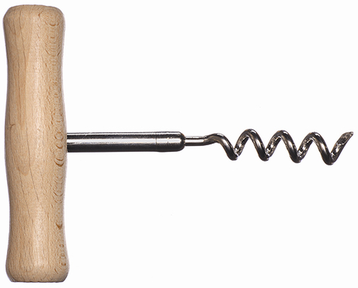
\includegraphics[]{corksckrew}};
			\draw [thick, red, decoration={
						markings,
						mark=at position 0.5 with {\arrow{latex}}}, postaction={decorate}](0,0) [partial ellipse
				=5:355:0.25 and 1];
			\draw[blue, -latex, thick] (1.5, 0) -- ++(1, 0) node[right, black] {};
			%			\node[blue] at (0.5,1) {$N$};
			%			\node[red] at (-0.5,1) {$S$};
		\end{tikzpicture}
		 &
		\begin{tikzpicture}[baseline={(0,0)}]
			\draw [thick, red, decoration={
						markings,
						mark=at position 0.5 with {\arrow{latex}}}, postaction={decorate}](0,0) [ partial ellipse =0:360:0.25 and
				1];
			\draw[blue, -latex, thick] (0, 0) -- +(1, 0) node[right, black] {$\vec{p}_m$};
			%			\node[blue] at (0.5,1) {$N$};
			%			\node[red] at (-0.5,1) {$S$};
		\end{tikzpicture}
	\end{tblr}
\end{frame}
% ===========================================================================

% ============================== Слайд ## ===================================
\begin{frame}{Магнітні та механічні моменти різних тіл}{}
	\begin{block}{}\justifying
		Відношення магнітного моменту зарядженого тіла, до його механічного моменту називається гіромагнітним відношенням:
	\end{block}
	\begin{tblr}{Q[c,m,mode=dmath]X[c, m]}
		\tcbhighmath{\vect{p}_m = \gamma \vect{L}.}
		                                                               &
		\SetCell[r=2,c=1]{c, m}
		\tikz[baseline, >=latex]{
			\def\R{0.8}
			\draw[ball color=red] (0,0) circle (\R);
			\draw[->, thick, blue] (0, {\R+0.01}) -- ++(0, 0.5) node[above] {$\vect{\omega}$};
			\draw[->] (0, {\R+0.25}) [partial ellipse=110:{360 + 70}:0.5 and 0.1];
		}                                                                \\
		\text{Для любих \alert{класичних} тіл}\ \gamma = \frac{Q}{2Mc} &
	\end{tblr}
	\begin{tblr}{
		colspec={Q[c, m, 1.7cm]X[c,m, mode=dmath]X[c,m, mode=dmath]X[c,m, mode=dmath]},
		row{1}={mode=text, font=\bfseries\small, fg=white, bg=cyan, font=\bfseries},
		hlines,
		vlines,
		}
		Тіло                      & Момент імпульсу                   & Магнітний момент         & Гіромагнітне відношення $\gamma$ \\
		Куля                      & \vect{L} = \frac25mR^2\vect\omega & \vect{p}_m =
		\frac1{5c}QR^2\vect\omega & \frac{Q}{2Mc}                                                                                   \\
		Електрон                  & L = \frac12\hbar                  & p_m = \frac{e}{2mc}\hbar & -\frac{e}{m_ec}
	\end{tblr}
\end{frame}
% ===========================================================================


% ============================== Слайд ## ===================================
\begin{frame}{Вектор-потенціал на далеких відстанях}{}
	\begin{columns}
		\begin{column}{0.3\linewidth}
			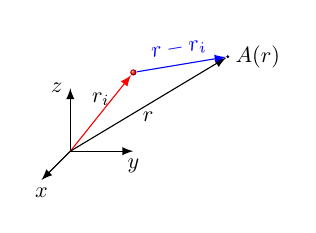
\begin{tikzpicture}[>=latex, scale=0.8, transform shape]
				\draw[->] (0,0) -- ++(1, 0) node[below] {$y$};
				\draw[->] (0,0) -- ++(0, 1) node[left] {$z$};
				\draw[->] (0,0) -- ++({180+45}:0.65) node[below] {$x$};

				\node[circle, inner sep=1pt, ball color=red] (i1) at (1, 1.25) {};
				\node[circle, inner sep=0.5, fill] (P) at (2.5, 1.5) {};
				\node[right] at (P) {$\vect{A}(\vect{r})$};

				\draw[->, red] (0,0) -- node[above, text=black] {$\vect{r}_i$} (i1);
				\draw[->] (0,0) -- node[below] {$\vect{r}$} (P);
				\draw[->, blue] (i1) -- node[above, sloped] {$\vect{r} - \vect{r}_i$} (P);
			\end{tikzpicture}
		\end{column}
		\begin{column}{0.7\linewidth}
			Магнітний момент системи тіл:
			\begin{equation*}
				\vect{A} = \frac1c \sum_i \frac{q_i\vect{v_i}}{|\vect{r} - \vect{r}_i|}
			\end{equation*}
		\end{column}
	\end{columns}
	\begin{overprint}
		\onslide<1>
		\begin{block}{}
			На далеких відстанях $r_i \ll r$ наближено
			\(
			\frac{1}{|\vect{r} - \vect{r}_i|} \approx \frac1r \left(1 + \frac{\vect{r}\ \vect{r}_i}{r^2}\right).
			\)
		\end{block}
		\begin{alertblock}{}\justifying\small
			Для стаціонарних рухів, які відбуваються в малих областях, можна зробити усереднення вектор-потенціалу, при цьому
			$\overline{\frac{d}{dt}\ldots}
				=
				0$.
		\end{alertblock}
		\begin{equation*}
			\overline{\vect{A}} = \frac1{cr^3} \sum_iq_i\overline{v_i(\vect{r}\ \vect{r}_i)}
		\end{equation*}
		\begin{center}\footnotesize
			\begin{equation*}
				v_i(\vect{r}\ \vect{r}_i) = \frac12\left[v_i(\vect{r}\ \vect{r}_i) - \vect{r}_i(\vect{r}\ \vect{v}_i)\right] +
				\frac12\left[v_i(\vect{r}\
					\vect{r}_i) + \vect{r}_i(\vect{r}\ \vect{v}_i)\right]
				= \frac12 \vect{r}\times\vect{v}_i\times\vect{r}_i + \frac12\frac{d}{dt}\left(\vect{r}_i(\vect{r}\ \vect{r}_i)\right).
			\end{equation*}
		\end{center}
		\onslide<2>
		\begin{equation*}
			\overline{\vect{A}} =  \frac1{r^3}  \left(\frac1{2c} \sum_i \vect{r}_i\times (q_i\vect{v}_i)\right)\times\vect{r} =
			\frac{\vect{p}_m\times\vect{r}}{r^3} .
		\end{equation*}
		Магнітне поле знаходиться за формулою $\Bfield = \Rot\vect{A}$:
		{\scriptsize%
		\begin{align*}
			\Rot\vecdot{\vect{A}}{\vect{B}}                                 & = \scdot{\vect{B}}{\grad}\vect{A} - \scdot{\vect{A}}{\grad}\vect{B}
			+ 	\vect{A}\Div\vect{B} -
			\vect{B}\Div\vect{A}
			\\
			\Bfield = \Rot\left(\vect{p}_m\times\frac{\vect{r}}{r^3}\right) &
			=
			%\cancelto{0}{\vect{p}_m\Div\frac{\vect{r}}{r^3}}
			-\scdot{\vect{p}_m}{\grad}\frac{\vect{r}}{r^3} = \frac{3\scdot{\vect{p}_m}{\vect{r}}\vect{r}}{r^5} - \frac{\vect{p}_m}{r^3}.
		\end{align*}
		}
		\begin{equation*}
			\Bfield = \frac{3\scdot{\vect{p}_m}{\vect{r}}\vect{r}}{r^5} - \frac{\vect{p}_m}{r^3}.
		\end{equation*}
	\end{overprint}
\end{frame}
% ===========================================================================






% ============================== Слайд ## ===================================
\begin{frame}{Детальние виведення}{}
	\thispagestyle{empty}
	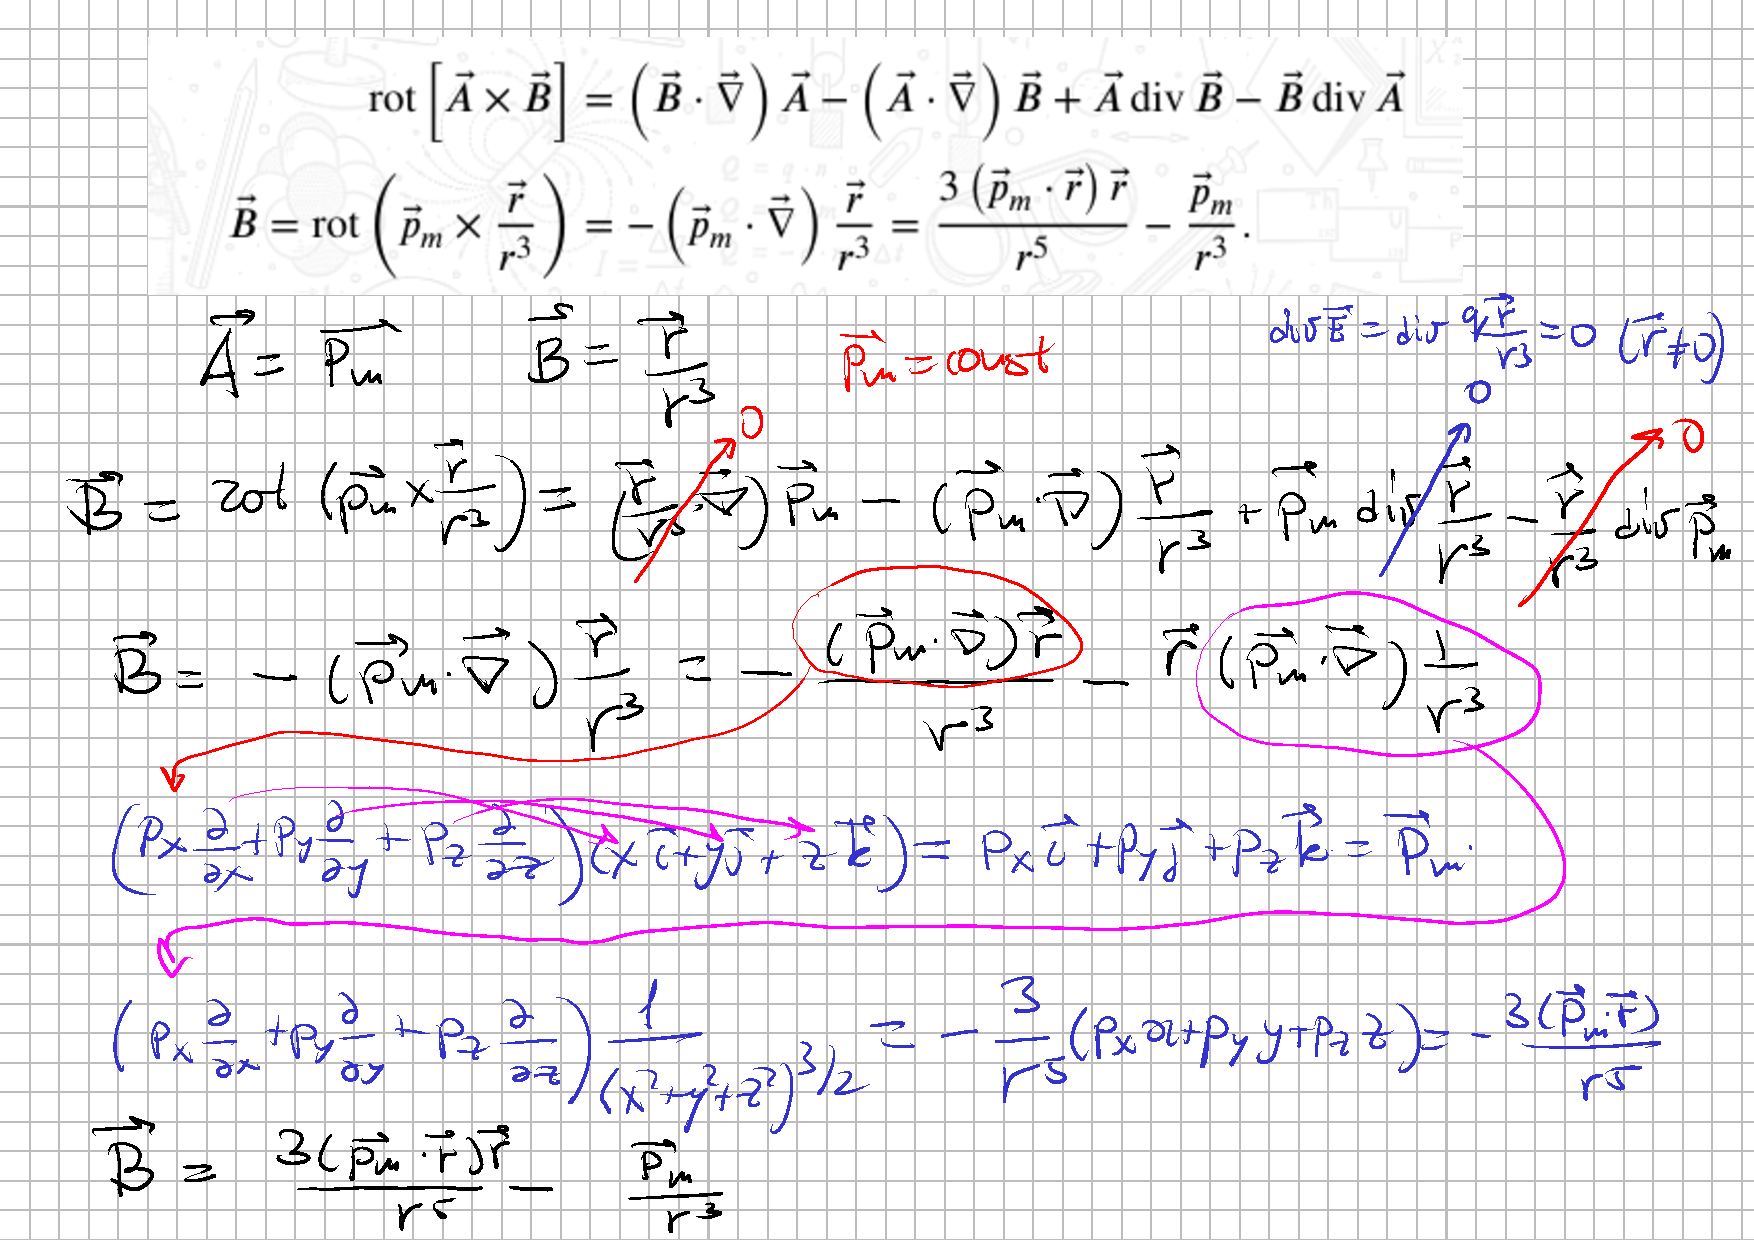
\includegraphics[width=\linewidth]{BrotA}
\end{frame}
% ===========================================================================






% ============================== Слайд ## ===================================
\begin{frame}{Магнітний диполь}{}
	\framesubtitle<1>{Полюса магніту}
	\begin{onlyenv}<1>
		\begin{block}{}
			Отримана формула збігається за виглядом із формулою для електричного поля точкового електричного диполя.
			\begin{equation*}
				\tcbhighmath{\Bfield = \frac{3\scdot{\vect{p}_m}{\vect{r}}\vect{r}}{r^5} - \frac{\vect{p}_m}{r^3}.}
			\end{equation*}
		\end{block}
		\begin{columns}
			\begin{column}{0.7\linewidth}
				\begin{block}{}\justifying
					Це означає, що точковий
					магнітний момент можна розглядати формально як точковий диполь, складений з \alert{\emph{ефективних магнітних зарядів}}:
					\begin{center}
						\textcolor{red}{$N$} (\textcolor{red}{північного}) та \textcolor{blue}{$S$} (\textcolor{blue}{південного}).
					\end{center}
				\end{block}
			\end{column}
			\begin{column}{0.3\linewidth}\centering
				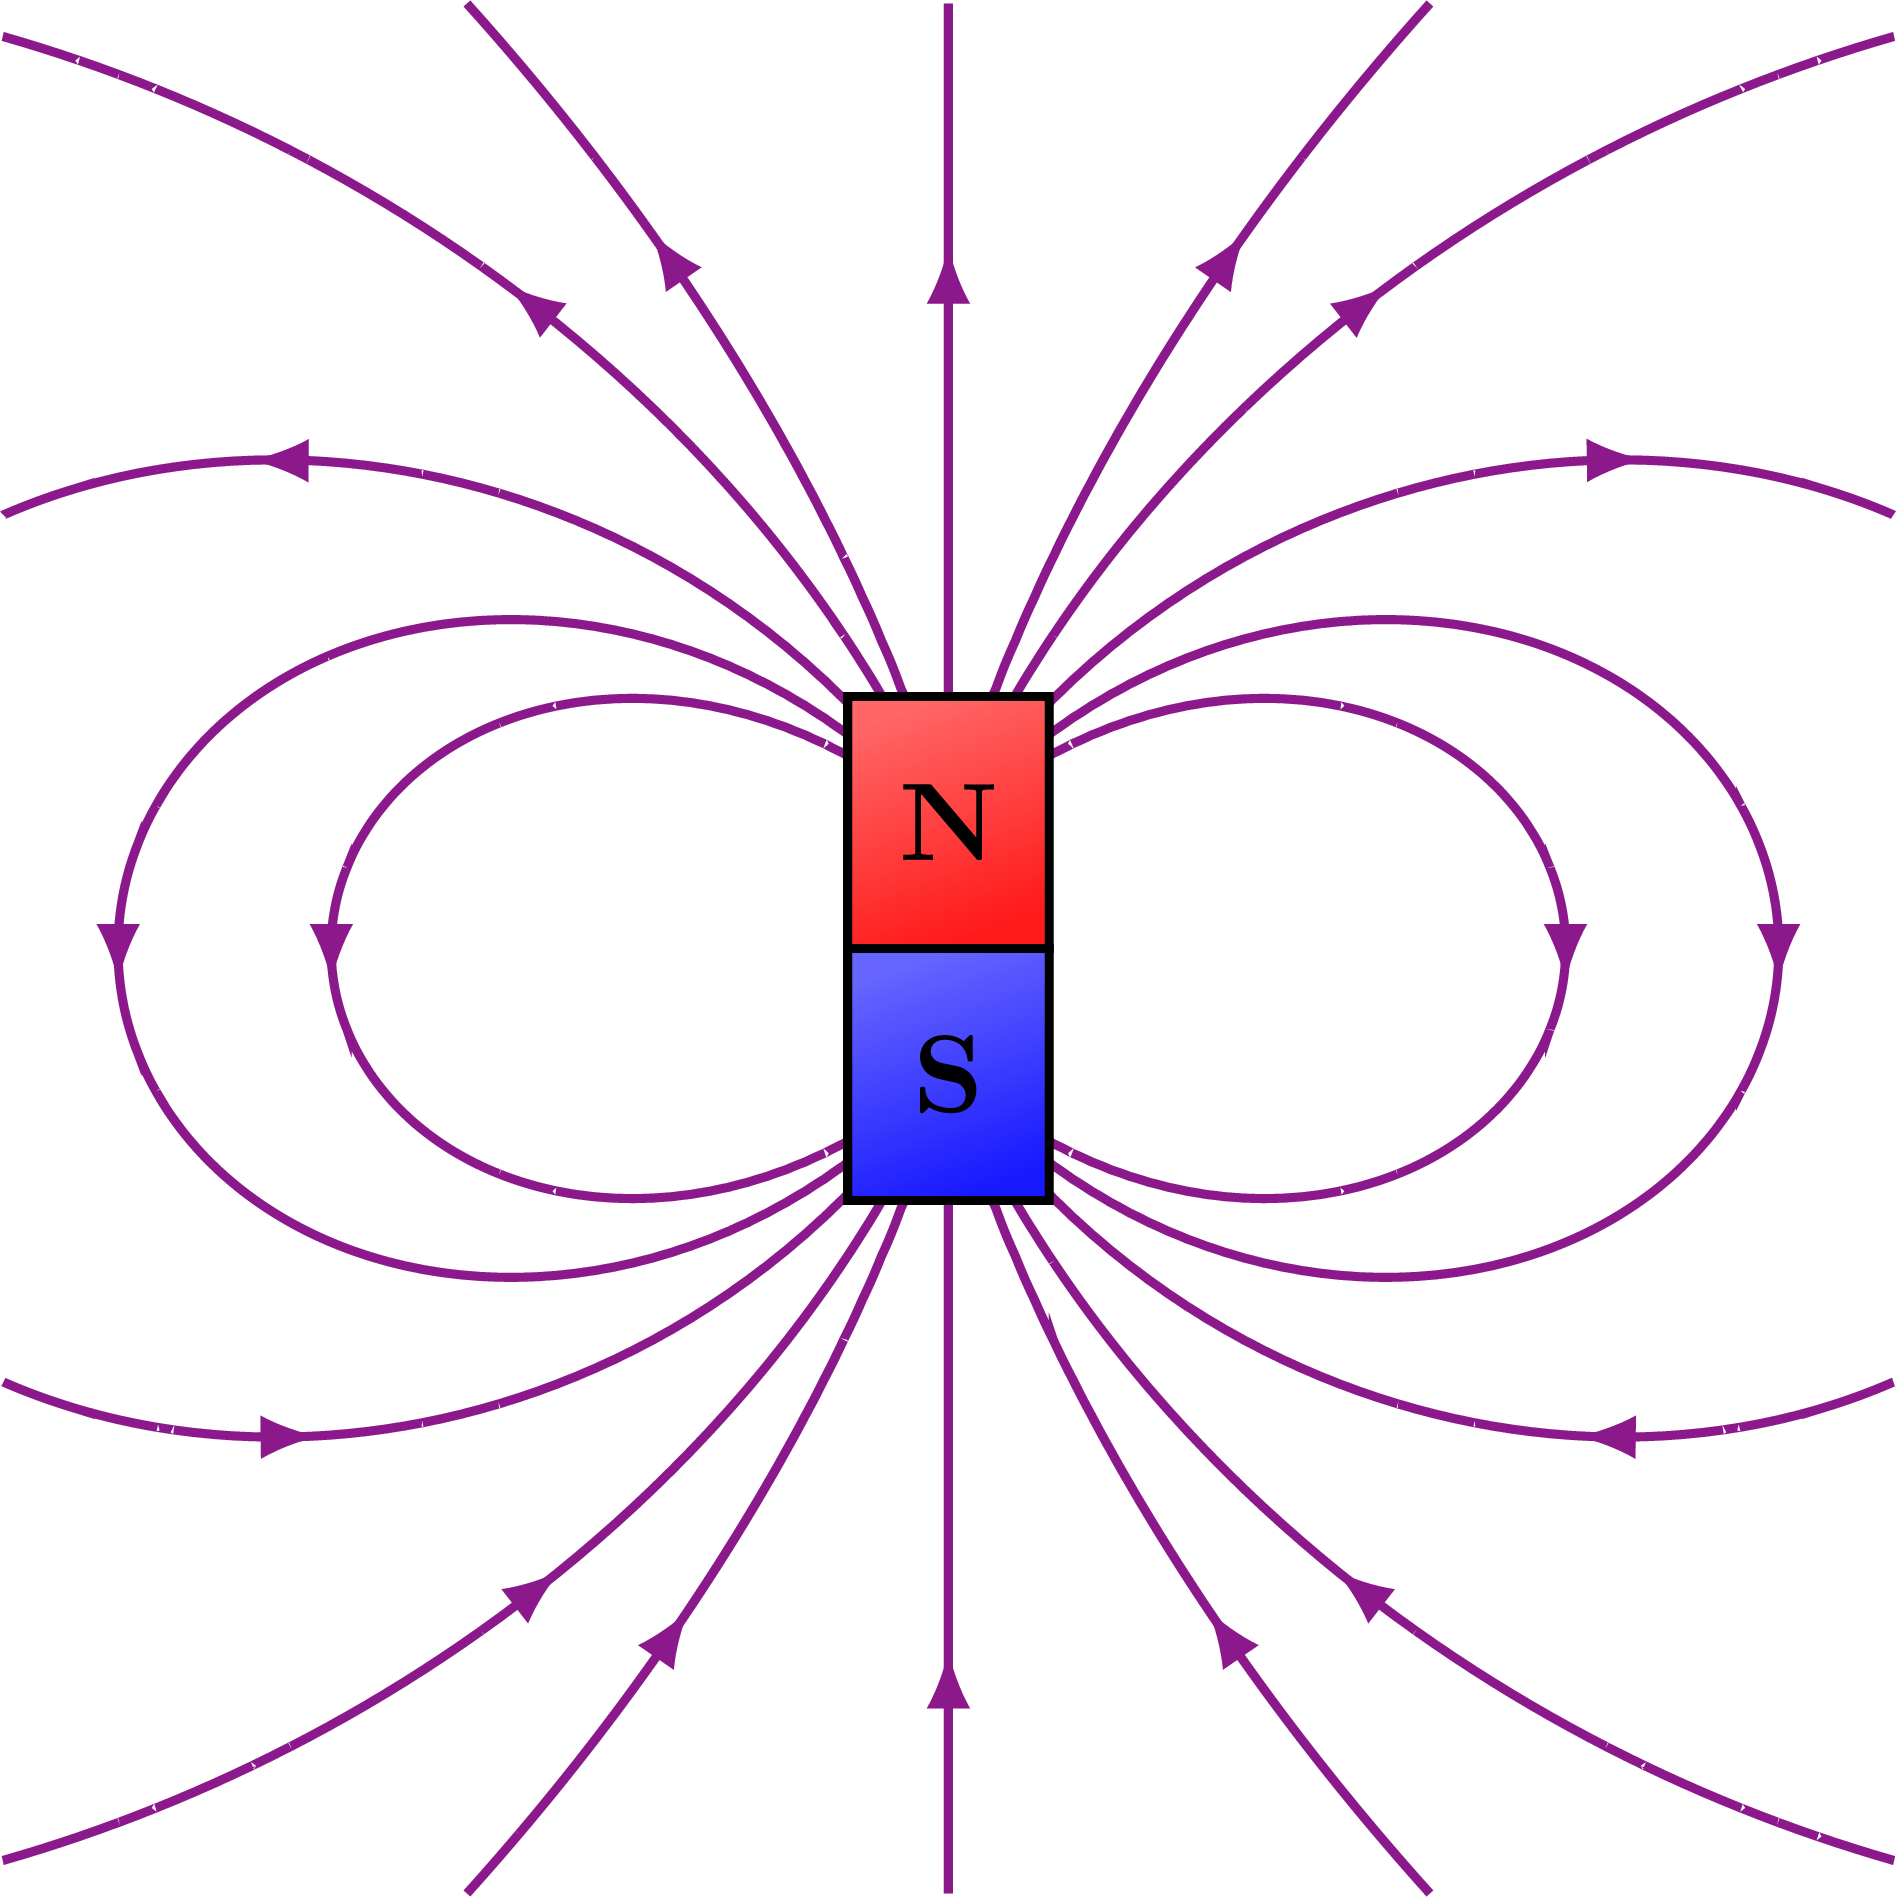
\includegraphics[width=\linewidth]{magdipole}
			\end{column}
		\end{columns}
	\end{onlyenv}
	\framesubtitle<2>{Порівняння електричного та магнітного диполів}
	\begin{onlyenv}<2>
		\begin{center}\small
			\begin{tblr}%
				{
				colspec={Q[l,m]X[c,m,bg=red! 10]X[c,m, bg=blue! 10]},
				cell{1}{2,3} = {fg=white, bg=cyan, font=\bfseries},
				cell{2,3}{1} = {bg=yellow!10, font=\bfseries},
						hlines,
						vlines,
					}
				          & Електричний диполь                                                                        & Магнітний
				диполь                                                                                                              \\
				%			Означення & $\vect{p}_e = \iiint\limits_V \rho dV$                                                  & $\vect{p}_m =
				%\frac1{2c}
				%\iiint\limits_V \vect{r}\times \rho\vect{v}\ dV$ \\
				Потенціал & $\phi = \dfrac{\vect{p}_e\cdot\vect{r}}{r^3}$                                             & $\vect{A} =
				\dfrac{\vect{p}_m\times\vect{r}}{r^3}$                                                                              \\
				Поле      & $\Efield = \dfrac{3\scdot{\vect{p}_e}{\vect{r}}\vect{r}}{r^5} - \dfrac{\vect{p}_e}{r^3} $ & $\Bfield =
					\dfrac{3\scdot{\vect{p}_m}{\vect{r}}\vect{r}}{r^5} -
				\dfrac{\vect{p}_m}{r^3}$                                                                                            \\
			\end{tblr}
		\end{center}
		\begin{columns}
			\begin{column}{0.7\linewidth}
				\begin{block}{}\justifying\small
					Позначаючи величину ефективного магнітного заряду $q_m$ і плече магнітного диполя $\vect{\ell}$, дипольний момент ефективного
					магнітного
					диполя можна
					записати як
					\(
					\vect{p}_m = q_m \vect{\ell}.
					\)
					Якщо не розглядати поле усередині такого магнітного диполя, то воно усюди буде таким самим, як і поле системи струмів із магнітним
					моментом
					$\vect{p}_m$.
				\end{block}
			\end{column}
			\begin{column}{0.3\linewidth}\centering
				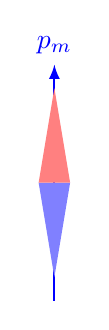
\begin{tikzpicture}[>=latex]
					\def\t{0.2}
					\def\h{1.2}
					\draw[->, blue, thick] (0, {-(\h+0.3)}) -- (0, {\h+0.3}) node[above] {$\vect{p}_m$};
					\fill[blue!50] (0, -\h) --  (-\t, 0) -- (\t, 0) -- cycle;
					\fill[red!50] (-\t, 0) -- (0, \h) -- (\t, 0) -- cycle;
					%                    \draw[->, ultra thin, white] (0, {-\h}) -- (0, \h);
				\end{tikzpicture}
			\end{column}
		\end{columns}
	\end{onlyenv}
\end{frame}
% ===========================================================================

%% --------------------------------------------------------
\section{Потенціальна енергія диполя та сила, що діє на диполь в магнітному полі}
%% --------------------------------------------------------



% ============================== Слайд ## ===================================
\begin{frame}{Момент сили, що діє на контур в магнітному полі}{}\footnotesize
	\begin{columns}
		\begin{column}{0.75\linewidth}
			\begin{block}{}\justifying
				Якщо виток перебуває в однорідному магнітному полі, то виникає момент сил, який орієнтує
				його магнітний момент за напрямком поля. За означенням моменту сил:
				\begin{equation*}
					\vect{M} = \frac1c \oint\limits_L  \vect{r}\times(Id\vect{\ell}\times\Bfield).
				\end{equation*}
			\end{block}
		\end{column}
		\begin{column}{0.25\linewidth}\centering
			\begin{tikzpicture}[>=latex]
				\foreach \x in {-2,...,2} {
						\draw[->, blue] ({0.6*\x}, -1.5) -- ++(0, 3);
					}

				\begin{scope}[rotate around={45:(0,0)}]
					\draw[->, thick, gray] (0, 1) -- ++(-45:-0.7) node[below=5pt, inner sep=1pt, fill=white] {$d\vect{F}$};
					\draw[->, thick, gray] (0, -1) -- ++(-45:0.7);
					\draw[arrowpos={0.5}{2pt}{7pt}, red!40, ultra thick] (0,0) [partial ellipse=0:360:0.3 and 1];
					\draw[red, ultra thick] (0,0) [partial ellipse=110:70:0.3 and 1];
					\draw[->,  thick] (0, 0) --  node[anchor=south west] {$\vect{r}'$} ++(0, 1);
				\end{scope}
			\end{tikzpicture}
		\end{column}
	\end{columns}
	\begin{block}{}\tiny
		\alert{Треба витягнути $\Bfield$ з-під інтегралу. Всі інтеграли типу $\oint\limits_L d(\ldots) = 0$, як інтеграли повних диференціалів.}
		\begin{equation*}
			\overset{\color{red}a}{\vect{r}}\times(\overset{\color{red}b}{d\vect{r}}\times\overset{\color{red}c}{\Bfield}) =
			\overset{\color{red}b}{d\vect{r}}\ (\overset{\color{red}a}{\vect{r}}\cdot\overset{\color{red}c}{\Bfield}) -
			\overset{\color{red}c}{\Bfield}\ (\overset{\color{red}a}{\vect{r}}\cdot\overset{\color{red}b}{d\vect{r}}), \
			\oint\limits_L  d\vect{r} (\vect{r}\cdot\Bfield)  - \cancelto{0}{\Bfield \oint\limits_L d\left(\frac{r^2}{2}\right)}
		\end{equation*}
		\begin{equation*}
			d\vect{r} (\vect{r}\cdot\Bfield) = \frac12 \left[d\vect{r} (\vect{r}\cdot\Bfield) + \vect{r} (d\vect{r}\cdot\Bfield) \right] +
			\frac12 \left[d\vect{r} (\vect{r}\cdot\Bfield) - \vect{r} (d\vect{r}\cdot\Bfield) \right] = \frac12 \left[d\vect{r} (\Bfield\cdot\vect{r}) +
				\vect{r} (\Bfield\cdot d\vect{r}) \right]  - \frac12 \Bfield\times(\vect{r}\times d\vect{r}).
		\end{equation*}
		\begin{equation*}
			d\vect{r} (\Bfield\cdot\vect{r}) +
			\vect{r} (\Bfield\cdot d\vect{r})  = d(\vect{r}(\Bfield\cdot\vect{r})),\
			\oint\limits_L d(\vect{r}(\Bfield\cdot\vect{r})) = 0.
		\end{equation*}
	\end{block}
	\begin{equation*}
		\vect{M} = \left(\frac{I}{c} \oint\limits_L (\vect{r}\times d\vect{r})\right)\times\Bfield = \vect{p}_m\times\Bfield
	\end{equation*}
\end{frame}
% ===========================================================================



% ============================== Слайд ## ===================================
\begin{frame}{Потенціальна енергія диполя в магнітному полі}{}
	\begin{block}{}\justifying
		Розглянемо виток площею $S$, у якому циркулює \alert{постійний} струм $I$. Магнітний момент цього витка $\vect{p}_m = \frac1c IS\ \vec{n}$.
		%Вважаємо, що магнітний
		%момент не змінюється за величиною, тільки може змінювати напрямок у просторі. Останнє припущення істотне, і воно передбачає, що в коло витка
		%ввімкнене
		%\alert{джерело ЕРС, що підтримує струм незмінним}.
	\end{block}

	\begin{columns}
		\begin{column}{0.75\linewidth}
			\begin{block}{}\justifying
				Якщо виток перебуває в однорідному магнітному полі, то виникає момент сил, які прагнуть орієнтувати
				його магнітний момент за напрямком поля:
				\begin{equation*}
					\vect{M} = \left[\vect{p}_m\times\Bfield\right]
				\end{equation*}
				З визначення потенціальної енергії знаходимо
				\begin{equation*}
					U = -\vect{p}_m\cdot\Bfield
				\end{equation*}
			\end{block}
		\end{column}
		\begin{column}{0.25\linewidth}\centering
			\begin{tikzpicture}[>=latex]
				\foreach \x in {-2,...,2} {
						\draw[->, blue] ({0.6*\x}, -1.5) -- ++(0, 3);
					}
				\begin{scope}[rotate around={0:(0,0)}, opacity=0.1]
					\draw[->, thick, gray] (0, 1) -- ++(-0.7, 0);
					\draw[->, thick, gray] (0, -1) -- ++(0.7, 0);
					\draw[arrowpos={0.5}{2pt}{7pt}, red, ultra thick] (0,0) [partial ellipse=0:360:0.3 and 1];
					\draw[->, brown, thick] (0, 0) -- ++(1, 0);
					\pic[opacity=0.1, rotate={180+0}, scale=0.7] at (0, 0) {magarrow};
				\end{scope}

				\begin{scope}[rotate around={45:(0,0)}]
					\draw[->, thick, gray] (0, 1) -- ++(-45:-0.7);
					\draw[->, thick, gray] (0, -1) -- ++(-45:0.7);
					\draw[arrowpos={0.5}{2pt}{7pt}, red, ultra thick] (0,0) [partial ellipse=0:360:0.3 and 1];
					\draw[->, brown, thick] (0, 0) -- ++(1, 0) node[anchor=south west] {$\vect{p}_m$};
					\pic[opacity=0.4, rotate={180+45}, scale=0.7] at (0, 0) {magarrow};
				\end{scope}
			\end{tikzpicture}
		\end{column}
	\end{columns}
	\begin{block}{}
		Той факт, що потенціальна енергія досягає мінімуму $\vect{p}_m\uparrow\uparrow\Bfield$, означає, що момент прагне орієнтуватися за напрямом
		поля.
	\end{block}

	\begin{alertblock}{}\justifying
		Якщо магнітний диполь представляє собою виток, через який тече постійний струм, і магнітне поле орієнтує його, то потенційна енергія витка
		змінюється. Однак, оскільки магнітне поле не є потенційним і не може виконувати роботу, постає питання: за рахунок чого відбувається зміна
		енергії
		витка?
		\href{https://chatgpt.com/share/671944e1-0220-8013-9fb3-11bfec044641}{\color{blue}Відповідь}
	\end{alertblock}

\end{frame}
% ===========================================================================





% ============================== Слайд ## ===================================
\begin{frame}{Принцип роботи електричного двигуна}{}

	\begin{columns}
		\begin{column}{0.4\linewidth}\centering\scriptsize
			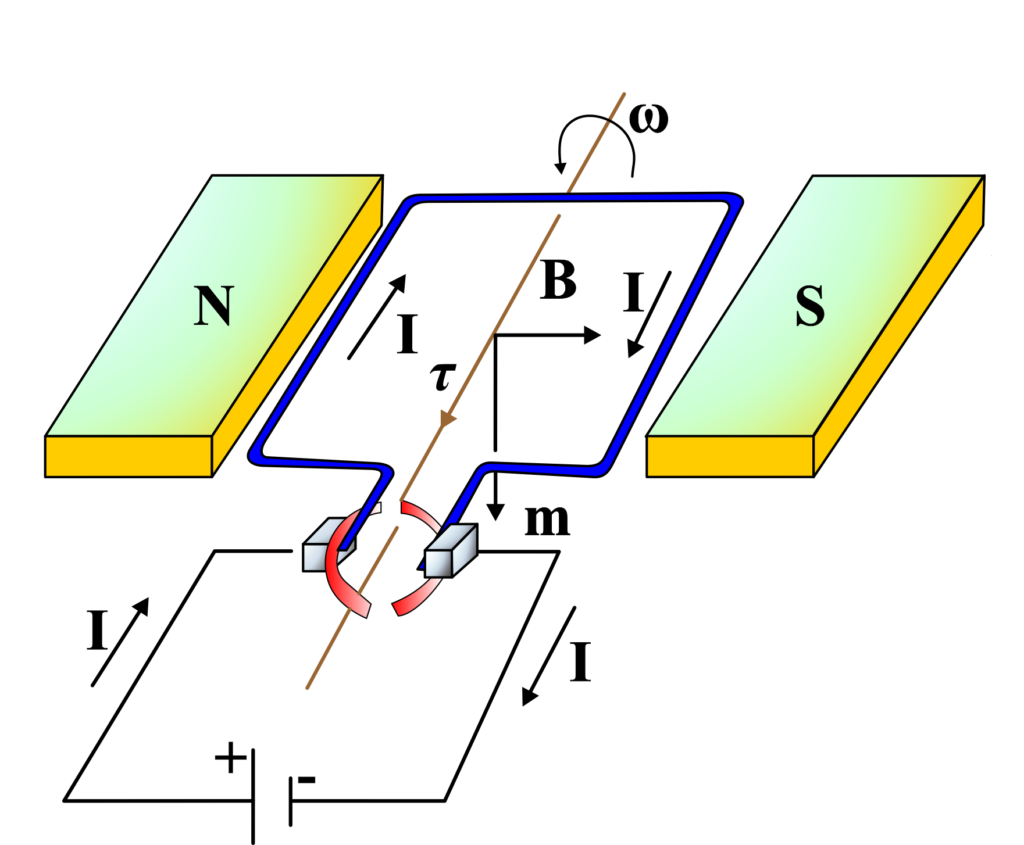
\includegraphics[width=1\linewidth]{motor}
		\end{column}
		\begin{column}{0.6\linewidth}
			\begin{block}{}\justifying
				На основі дії магнітного поля на рамку, через яку проходить електричний струм, ґрунтується принцип роботи електродвигуна.
			\end{block}
			\begin{alertblock}{}\justifying\small
				Робота по обертанню рамки виконується не магнітним полем, а за рахунок енергії джерела. Роль магнітного полягає у тому, щоб
				перенаправити цю енергію у механічну, а саме у обертання рамки.
			\end{alertblock}
		\end{column}
	\end{columns}
	\begin{block}{}\scriptsize
		\begin{enumerate}
			\item Ротор (провідник), через який тече струм, поміщений у зовнішнє магнітне поле між полюсами магнітів (N і S).
			\item Відповідно до правила лівої руки, на провідник діє сила з боку магнітного поля (сила Ампера), що створює обертальний момент.
			\item Магнітний момент системи намагається вирівнятися з напрямом зовнішнього поля.
			\item Комутатор змінює напрям струму в обмотці після кожного півоберта, забезпечуючи постійне обертання у одному напрямку.
		\end{enumerate}
	\end{block}
\end{frame}
% ===========================================================================




% ============================== Слайд ## ===================================
\begin{frame}{Сила, що діє на диполь в магнітному полі}{}\small
	\begin{block}{}\justifying
		У зовнішньому магнітному полі потенціальна енергія магнітного моменту дорівнює $U = -\vect{p}_m\cdot\Bfield$, а сила, що діє на
		момент:
		\begin{equation*}
			\vect{F} = -\grad U = \grad(\vect{p}_m\cdot\Bfield).
		\end{equation*}
	\end{block}
	\begin{columns}
		\begin{column}{0.75\linewidth}
			\begin{block}{}\justifying
				У зовнішньому магнітному полі потенціальна енергія магнітного моменту дорівнює $U = -\vect{p}_m\cdot\Bfield$, а сила, що діє на
				момент:
				\begin{equation*}
					\vect{F} = -\grad U = \grad(\vect{p}_m\cdot\Bfield).
				\end{equation*}
				{\scriptsize \begin{equation*}
					\grad\scdot{\vect{A}}{\vect{B}}  = \vecdot{\vect{B}}{\Rot\vect{A}} + \vecdot{\vect{A}}{\Rot\vect{B}} +
					\scdot{\vect{B}}{\grad}\vect{A} +
					\scdot{\vect{A}}{\grad}\vect{B}.
				\end{equation*}}

				Якщо в середовищі, в якому перебуває момент, відсутні струми провідності, то $\Rot\Bfield = 0$. Тоді має місце тотожність:
				\begin{equation*}
					\tcbhighmath{\vect{F} = \scdot{\vect{p}_m}{\grad}\vect{B}.}
				\end{equation*}
			\end{block}
		\end{column}
		\begin{column}{0.25\linewidth}\centering
			\begin{tikzpicture}[scale=0.9, >=latex, midarrow/.style={%
							postaction={ decorate,
									decoration={ markings, mark=at position .7 with {\arrow{latex}}}}}]

				\foreach \y in {-3,...,3}{
						\draw[blue, midarrow] plot[domain=1:4] (\x, 0.2*\y+0.05*\y*\x^2);
					}

				\coordinate (AP) at (3, 0);
				\pic[scale=0.7, rotate=210] at (AP) {magarrow};
				\draw[->, ultra thick] (AP) -- ++(-1, 0) node[below=2pt, fill=white, inner sep=1pt] {$\vect{F}$};
			\end{tikzpicture}
		\end{column}
	\end{columns}
	%	\begin{block}{}\justifying\scriptsize
	%		У окремому випадку, коли момент спрямований уздовж поля $\vect{p}_m\uparrow\uparrow\vect{B}$, а поле залежить тільки від координати
	%		$z$, сила
	%		спрямована по осі $z$ і дорівнює:
	%		\begin{equation*}
	%			F_z = p_m\frac{dB}{dz}.
	%		\end{equation*}
	%	\end{block}
	%	\href{https://www.youtube.com/watch?v=66yHf8Mv1SQ}{\scriptsize\color{blue} Порівняйте з випадком електричного диполя в неоднорідному електричному
	%		полі}
\end{frame}
% ===========================================================================
% https://tikz.net/magnetic_moment/


\end{document}
